\documentclass[twoside]{book}

% Packages required by doxygen
\usepackage{fixltx2e}
\usepackage{calc}
\usepackage{doxygen}
\usepackage[export]{adjustbox} % also loads graphicx
\usepackage{graphicx}
\usepackage[utf8]{inputenc}
\usepackage{makeidx}
\usepackage{multicol}
\usepackage{multirow}
\PassOptionsToPackage{warn}{textcomp}
\usepackage{textcomp}
\usepackage[nointegrals]{wasysym}
\usepackage[table]{xcolor}

% Font selection
\usepackage[T1]{fontenc}
\usepackage[scaled=.90]{helvet}
\usepackage{courier}
\usepackage{amssymb}
\usepackage{sectsty}
\renewcommand{\familydefault}{\sfdefault}
\allsectionsfont{%
  \fontseries{bc}\selectfont%
  \color{darkgray}%
}
\renewcommand{\DoxyLabelFont}{%
  \fontseries{bc}\selectfont%
  \color{darkgray}%
}
\newcommand{\+}{\discretionary{\mbox{\scriptsize$\hookleftarrow$}}{}{}}

% Page & text layout
\usepackage{geometry}
\geometry{%
  a4paper,%
  top=2.5cm,%
  bottom=2.5cm,%
  left=2.5cm,%
  right=2.5cm%
}
\tolerance=750
\hfuzz=15pt
\hbadness=750
\setlength{\emergencystretch}{15pt}
\setlength{\parindent}{0cm}
\setlength{\parskip}{3ex plus 2ex minus 2ex}
\makeatletter
\renewcommand{\paragraph}{%
  \@startsection{paragraph}{4}{0ex}{-1.0ex}{1.0ex}{%
    \normalfont\normalsize\bfseries\SS@parafont%
  }%
}
\renewcommand{\subparagraph}{%
  \@startsection{subparagraph}{5}{0ex}{-1.0ex}{1.0ex}{%
    \normalfont\normalsize\bfseries\SS@subparafont%
  }%
}
\makeatother

% Headers & footers
\usepackage{fancyhdr}
\pagestyle{fancyplain}
\fancyhead[LE]{\fancyplain{}{\bfseries\thepage}}
\fancyhead[CE]{\fancyplain{}{}}
\fancyhead[RE]{\fancyplain{}{\bfseries\leftmark}}
\fancyhead[LO]{\fancyplain{}{\bfseries\rightmark}}
\fancyhead[CO]{\fancyplain{}{}}
\fancyhead[RO]{\fancyplain{}{\bfseries\thepage}}
\fancyfoot[LE]{\fancyplain{}{}}
\fancyfoot[CE]{\fancyplain{}{}}
\fancyfoot[RE]{\fancyplain{}{\bfseries\scriptsize Generated by Doxygen }}
\fancyfoot[LO]{\fancyplain{}{\bfseries\scriptsize Generated by Doxygen }}
\fancyfoot[CO]{\fancyplain{}{}}
\fancyfoot[RO]{\fancyplain{}{}}
\renewcommand{\footrulewidth}{0.4pt}
\renewcommand{\chaptermark}[1]{%
  \markboth{#1}{}%
}
\renewcommand{\sectionmark}[1]{%
  \markright{\thesection\ #1}%
}

% Indices & bibliography
\usepackage{natbib}
\usepackage[titles]{tocloft}
\setcounter{tocdepth}{3}
\setcounter{secnumdepth}{5}
\makeindex

% Hyperlinks (required, but should be loaded last)
\usepackage{ifpdf}
\ifpdf
  \usepackage[pdftex,pagebackref=true]{hyperref}
\else
  \usepackage[ps2pdf,pagebackref=true]{hyperref}
\fi
\hypersetup{%
  colorlinks=true,%
  linkcolor=blue,%
  citecolor=blue,%
  unicode%
}

% Custom commands
\newcommand{\clearemptydoublepage}{%
  \newpage{\pagestyle{empty}\cleardoublepage}%
}

\usepackage{caption}
\captionsetup{labelsep=space,justification=centering,font={bf},singlelinecheck=off,skip=4pt,position=top}

%===== C O N T E N T S =====

\begin{document}

% Titlepage & ToC
\hypersetup{pageanchor=false,
             bookmarksnumbered=true,
             pdfencoding=unicode
            }
\pagenumbering{alph}
\begin{titlepage}
\vspace*{7cm}
\begin{center}%
{\Large as }\\
\vspace*{1cm}
{\large Generated by Doxygen 1.8.13}\\
\end{center}
\end{titlepage}
\clearemptydoublepage
\pagenumbering{roman}
\tableofcontents
\clearemptydoublepage
\pagenumbering{arabic}
\hypersetup{pageanchor=true}

%--- Begin generated contents ---
\chapter{Namespace Index}
\section{Namespace List}
Here is a list of all namespaces with brief descriptions\+:\begin{DoxyCompactList}
\item\contentsline{section}{\hyperlink{namespaceas}{as} }{\pageref{namespaceas}}{}
\item\contentsline{section}{\hyperlink{namespaceas_1_1console}{as\+::console} }{\pageref{namespaceas_1_1console}}{}
\item\contentsline{section}{\hyperlink{namespaceas_1_1details}{as\+::details} }{\pageref{namespaceas_1_1details}}{}
\item\contentsline{section}{\hyperlink{namespaceas_1_1graph}{as\+::graph} }{\pageref{namespaceas_1_1graph}}{}
\item\contentsline{section}{\hyperlink{namespaceas_1_1tmp}{as\+::tmp} }{\pageref{namespaceas_1_1tmp}}{}
\item\contentsline{section}{\hyperlink{namespaceas_1_1tmp_1_1details}{as\+::tmp\+::details} }{\pageref{namespaceas_1_1tmp_1_1details}}{}
\item\contentsline{section}{\hyperlink{namespaceconsole}{console} \\*This namespace contains miscellaneous console utilities }{\pageref{namespaceconsole}}{}
\item\contentsline{section}{\hyperlink{namespacegraph}{graph} \\*This namespace provides functions which work with boost graphs }{\pageref{namespacegraph}}{}
\item\contentsline{section}{\hyperlink{namespacetmp}{tmp} \\*Template-\/meta-\/programming namespace }{\pageref{namespacetmp}}{}
\end{DoxyCompactList}

\chapter{Hierarchical Index}
\section{Class Hierarchy}
This inheritance list is sorted roughly, but not completely, alphabetically\+:\begin{DoxyCompactList}
\item \contentsline{section}{as\+:\+:and\+\_\+die}{\pageref{structas_1_1and__die}}{}
\item false\+\_\+type\begin{DoxyCompactList}
\item \contentsline{section}{as\+:\+:tmp\+:\+:details\+:\+:can\+\_\+apply$<$ Z, types, class $>$}{\pageref{structas_1_1tmp_1_1details_1_1can__apply}}{}
\item \contentsline{section}{as\+:\+:tmp\+:\+:details\+:\+:is\+\_\+associative$<$ class, class $>$}{\pageref{structas_1_1tmp_1_1details_1_1is__associative}}{}
\end{DoxyCompactList}
\item \contentsline{section}{as\+:\+:iterator\+\_\+pair$<$ Iterator $>$}{\pageref{classas_1_1iterator__pair}}{}
\item true\+\_\+type\begin{DoxyCompactList}
\item \contentsline{section}{as\+:\+:tmp\+:\+:details\+:\+:can\+\_\+apply$<$ Z, types$<$ Ts... $>$, std\+:\+:void\+\_\+t$<$ Z$<$ Ts... $>$ $>$ $>$}{\pageref{structas_1_1tmp_1_1details_1_1can__apply_3_01Z_00_01types_3_01Ts_8_8_8_01_4_00_01std_1_1void__t_d0380c4f39b26cf3dcf2ed45500ba357}}{}
\item \contentsline{section}{as\+:\+:tmp\+:\+:details\+:\+:is\+\_\+associative$<$ Container, std\+:\+:void\+\_\+t$<$ typename Container\+:\+:key\+\_\+type $>$ $>$}{\pageref{structas_1_1tmp_1_1details_1_1is__associative_3_01Container_00_01std_1_1void__t_3_01typename_01Container_1_1key__type_01_4_01_4}}{}
\end{DoxyCompactList}
\item \contentsline{section}{as\+:\+:tmp\+:\+:types$<$... $>$}{\pageref{structas_1_1tmp_1_1types}}{}
\end{DoxyCompactList}

\chapter{Class Index}
\section{Class List}
Here are the classes, structs, unions and interfaces with brief descriptions\+:\begin{DoxyCompactList}
\item\contentsline{section}{\hyperlink{structas_1_1and__die}{as\+::and\+\_\+die} \\*A struct used to signal that the programme should be terminated immediately (die) }{\pageref{structas_1_1and__die}}{}
\item\contentsline{section}{\hyperlink{structas_1_1tmp_1_1details_1_1can__apply}{as\+::tmp\+::details\+::can\+\_\+apply$<$ Z, types, class $>$} }{\pageref{structas_1_1tmp_1_1details_1_1can__apply}}{}
\item\contentsline{section}{\hyperlink{structas_1_1tmp_1_1details_1_1can__apply_3_01Z_00_01types_3_01Ts_8_8_8_01_4_00_01std_1_1void__t_d0380c4f39b26cf3dcf2ed45500ba357}{as\+::tmp\+::details\+::can\+\_\+apply$<$ Z, types$<$ Ts... $>$, std\+::void\+\_\+t$<$ Z$<$ Ts... $>$ $>$ $>$} }{\pageref{structas_1_1tmp_1_1details_1_1can__apply_3_01Z_00_01types_3_01Ts_8_8_8_01_4_00_01std_1_1void__t_d0380c4f39b26cf3dcf2ed45500ba357}}{}
\item\contentsline{section}{\hyperlink{structas_1_1tmp_1_1details_1_1is__associative}{as\+::tmp\+::details\+::is\+\_\+associative$<$ class, class $>$} }{\pageref{structas_1_1tmp_1_1details_1_1is__associative}}{}
\item\contentsline{section}{\hyperlink{structas_1_1tmp_1_1details_1_1is__associative_3_01Container_00_01std_1_1void__t_3_01typename_01Container_1_1key__type_01_4_01_4}{as\+::tmp\+::details\+::is\+\_\+associative$<$ Container, std\+::void\+\_\+t$<$ typename Container\+::key\+\_\+type $>$ $>$} }{\pageref{structas_1_1tmp_1_1details_1_1is__associative_3_01Container_00_01std_1_1void__t_3_01typename_01Container_1_1key__type_01_4_01_4}}{}
\item\contentsline{section}{\hyperlink{classas_1_1iterator__pair}{as\+::iterator\+\_\+pair$<$ Iterator $>$} \\*This class wraps a pair of begin and end iterators, and exposes them via \hyperlink{classas_1_1iterator__pair_a88c00afafd5ee4477b7ab2a1a89bb746}{begin()} and \hyperlink{classas_1_1iterator__pair_ae7cef6e91faecd20e6aebd2f21b29b41}{end()} function, which can be used in range-\/based for loops }{\pageref{classas_1_1iterator__pair}}{}
\item\contentsline{section}{\hyperlink{structas_1_1tmp_1_1types}{as\+::tmp\+::types$<$... $>$} }{\pageref{structas_1_1tmp_1_1types}}{}
\end{DoxyCompactList}

\chapter{File Index}
\section{File List}
Here is a list of all files with brief descriptions\+:\begin{DoxyCompactList}
\item\contentsline{section}{src/\hyperlink{and__die_8h}{and\+\_\+die.\+h} }{\pageref{and__die_8h}}{}
\item\contentsline{section}{src/\hyperlink{as__version_8h}{as\+\_\+version.\+h} \\*Keeps track of the as library major, minor, and build version numbers }{\pageref{as__version_8h}}{}
\item\contentsline{section}{src/\hyperlink{can__apply_8h}{can\+\_\+apply.\+h} }{\pageref{can__apply_8h}}{}
\item\contentsline{section}{src/\hyperlink{console_8h}{console.\+h} }{\pageref{console_8h}}{}
\item\contentsline{section}{src/\hyperlink{containers_8h}{containers.\+h} }{\pageref{containers_8h}}{}
\item\contentsline{section}{src/\hyperlink{file__stream_8h}{file\+\_\+stream.\+h} }{\pageref{file__stream_8h}}{}
\item\contentsline{section}{src/\hyperlink{graph_8h}{graph.\+h} }{\pageref{graph_8h}}{}
\item\contentsline{section}{src/\hyperlink{is__associative_8h}{is\+\_\+associative.\+h} }{\pageref{is__associative_8h}}{}
\item\contentsline{section}{src/\hyperlink{iterator__pair_8h}{iterator\+\_\+pair.\+h} }{\pageref{iterator__pair_8h}}{}
\end{DoxyCompactList}

\chapter{Namespace Documentation}
\hypertarget{namespaceas}{}\section{as Namespace Reference}
\label{namespaceas}\index{as@{as}}
\subsection*{Namespaces}
\begin{DoxyCompactItemize}
\item 
 \hyperlink{namespaceas_1_1console}{console}
\item 
 \hyperlink{namespaceas_1_1details}{details}
\item 
 \hyperlink{namespaceas_1_1graph}{graph}
\item 
 \hyperlink{namespaceas_1_1tmp}{tmp}
\end{DoxyCompactItemize}
\subsection*{Classes}
\begin{DoxyCompactItemize}
\item 
struct \hyperlink{structas_1_1and__die}{and\+\_\+die}
\begin{DoxyCompactList}\small\item\em A struct used to signal that the programme should be terminated immediately (die). \end{DoxyCompactList}\item 
class \hyperlink{classas_1_1iterator__pair}{iterator\+\_\+pair}
\begin{DoxyCompactList}\small\item\em This class wraps a pair of begin and end iterators, and exposes them via \hyperlink{classas_1_1iterator__pair_a88c00afafd5ee4477b7ab2a1a89bb746}{begin()} and \hyperlink{classas_1_1iterator__pair_ae7cef6e91faecd20e6aebd2f21b29b41}{end()} function, which can be used in range-\/based for loops. \end{DoxyCompactList}\end{DoxyCompactItemize}
\subsection*{Typedefs}
\begin{DoxyCompactItemize}
\item 
{\footnotesize template$<$class Container , class T $>$ }\\using \hyperlink{namespaceas_a9bd788709567003423247a9db4ba1074}{count\+\_\+method\+\_\+type} = decltype(std\+::declval$<$ Container $>$().count(std\+::declval$<$ T $>$()))
\begin{DoxyCompactList}\small\item\em This is the type of a generic .count() method for a container. \end{DoxyCompactList}\item 
{\footnotesize template$<$class Container , class T $>$ }\\using \hyperlink{namespaceas_a9e0fcaa3ddb46647d8979282465685da}{has\+\_\+count\+\_\+method} = \hyperlink{namespaceas_1_1tmp_a44a275bd3c66d727fb1b6f0179d49e19}{tmp\+::can\+\_\+apply}$<$ \hyperlink{namespaceas_a9bd788709567003423247a9db4ba1074}{count\+\_\+method\+\_\+type}, Container, T $>$
\begin{DoxyCompactList}\small\item\em This will inherit from true\+\_\+type iff class Container has an appopriate .count() method. \end{DoxyCompactList}\end{DoxyCompactItemize}
\subsection*{Functions}
\begin{DoxyCompactItemize}
\item 
std\+::ostream \& \hyperlink{namespaceas_a4d891ae352512e1c506d6cd01ff1422c}{operator$<$$<$} (std\+::ostream \&out, const \hyperlink{structas_1_1and__die}{and\+\_\+die} \&)
\begin{DoxyCompactList}\small\item\em Concatenates a \hyperlink{structas_1_1and__die}{and\+\_\+die} structure to an output stream, to immediately terminate a programme. \end{DoxyCompactList}\item 
{\footnotesize template$<$class Container , class T $>$ }\\bool \hyperlink{namespaceas_a49cf7ae4239ab51e54f099d30a84811a}{contains} (const Container \&container, const T \&element)
\begin{DoxyCompactList}\small\item\em Tells whether a container contains a certain element. \end{DoxyCompactList}\item 
{\footnotesize template$<$class Container $>$ }\\void \hyperlink{namespaceas_aab6569c28591bebed9bd29b40c772bfc}{join\+\_\+and\+\_\+print} (const Container \&container, std\+::ostream \&out=std\+::cout, std\+::string separator=\char`\"{}, \char`\"{})
\begin{DoxyCompactList}\small\item\em Joins the elements of a container using the separator, and prints the result to an output stream. \end{DoxyCompactList}\item 
void \hyperlink{namespaceas_a359f2d209e5ec052ec0d2752a589802d}{skip\+\_\+lines} (std\+::ifstream \&stream, std\+::size\+\_\+t how\+\_\+many=1u)
\begin{DoxyCompactList}\small\item\em Skips a certain number of lines from an input file stream. \end{DoxyCompactList}\item 
{\footnotesize template$<$class Iterator $>$ }\\\hyperlink{classas_1_1iterator__pair}{iterator\+\_\+pair}$<$ Iterator $>$ \hyperlink{namespaceas_a4d4e0fb99b7cc564adaa85b693392070}{make\+\_\+iter} (std\+::pair$<$ Iterator, Iterator $>$ iters)
\begin{DoxyCompactList}\small\item\em Gives an \hyperlink{classas_1_1iterator__pair}{iterator\+\_\+pair} object constructed from the beginning and end iterators, given as a pair. \end{DoxyCompactList}\item 
std\+::mt19937 \hyperlink{namespaceas_a4c9b0919bddf60796e9cc81ecd7d5bb2}{get\+\_\+seeded\+\_\+mt} ()
\begin{DoxyCompactList}\small\item\em Gets a properly seeded Mersenne Twister prng. \end{DoxyCompactList}\item 
{\footnotesize template$<$class Container , class Prng  = std\+::mt19937$>$ }\\Container \hyperlink{namespaceas_a001b8303767234a8c93de5cb530a8f3d}{sample} (const Container container, typename Container\+::size\+\_\+type how\+\_\+many, Prng \&\&prng)
\begin{DoxyCompactList}\small\item\em Gets samples from a container. The samples are guaranteed to be unique. If we are requesting more samples than elements in the container, the request is ignored, and instead a random permutation of the container is returned. \end{DoxyCompactList}\item 
{\footnotesize template$<$class Container $>$ }\\Container \hyperlink{namespaceas_ab2b3e64b4dee388f0ec34e41ae0b3e98}{sample} (const Container container, typename Container\+::size\+\_\+type how\+\_\+many)
\begin{DoxyCompactList}\small\item\em Gets samples from a container. The samples are guaranteed to be unique. If we are requesting more samples than elements in the container, the request is ignored, and instead a random permutation of the container is returned. \end{DoxyCompactList}\end{DoxyCompactItemize}


\subsection{Typedef Documentation}
\mbox{\Hypertarget{namespaceas_a9bd788709567003423247a9db4ba1074}\label{namespaceas_a9bd788709567003423247a9db4ba1074}} 
\index{as@{as}!count\+\_\+method\+\_\+type@{count\+\_\+method\+\_\+type}}
\index{count\+\_\+method\+\_\+type@{count\+\_\+method\+\_\+type}!as@{as}}
\subsubsection{\texorpdfstring{count\+\_\+method\+\_\+type}{count\_method\_type}}
{\footnotesize\ttfamily template$<$class Container , class T $>$ \\
using \hyperlink{namespaceas_a9bd788709567003423247a9db4ba1074}{as\+::count\+\_\+method\+\_\+type} = typedef decltype(std\+::declval$<$Container$>$().count(std\+::declval$<$T$>$()))}



This is the type of a generic .count() method for a container. 

count\+\_\+method\+\_\+type This method is implemented in some stl containers and takes an element as its only parameter. \mbox{\Hypertarget{namespaceas_a9e0fcaa3ddb46647d8979282465685da}\label{namespaceas_a9e0fcaa3ddb46647d8979282465685da}} 
\index{as@{as}!has\+\_\+count\+\_\+method@{has\+\_\+count\+\_\+method}}
\index{has\+\_\+count\+\_\+method@{has\+\_\+count\+\_\+method}!as@{as}}
\subsubsection{\texorpdfstring{has\+\_\+count\+\_\+method}{has\_count\_method}}
{\footnotesize\ttfamily template$<$class Container , class T $>$ \\
\hyperlink{namespaceas_a9e0fcaa3ddb46647d8979282465685da}{as\+::has\+\_\+count\+\_\+method}}



This will inherit from true\+\_\+type iff class Container has an appopriate .count() method. 



\subsection{Function Documentation}
\mbox{\Hypertarget{namespaceas_a49cf7ae4239ab51e54f099d30a84811a}\label{namespaceas_a49cf7ae4239ab51e54f099d30a84811a}} 
\index{as@{as}!contains@{contains}}
\index{contains@{contains}!as@{as}}
\subsubsection{\texorpdfstring{contains()}{contains()}}
{\footnotesize\ttfamily template$<$class Container , class T $>$ \\
bool as\+::contains (\begin{DoxyParamCaption}\item[{const Container \&}]{container,  }\item[{const T \&}]{element }\end{DoxyParamCaption})\hspace{0.3cm}{\ttfamily [inline]}}



Tells whether a container contains a certain element. 

The standard library\textquotesingle{}s functions to find elements (e.\+g. std\+::find) always return an iterator. Sometimes, though, we just want to know whether an element is in a container or not. This helper function lets us do this in a concise way. This function also has specialisation for when the container implements a .count() method, i.\+e. a more efficient way of searching elements than simple linear search.


\begin{DoxyTemplParams}{Template Parameters}
{\em Container} & Container type. \\
\hline
{\em T} & Containee type. \\
\hline
\end{DoxyTemplParams}

\begin{DoxyParams}{Parameters}
{\em container} & The container. \\
\hline
{\em element} & The element we are searching in {\ttfamily container}. \\
\hline
\end{DoxyParams}
\begin{DoxyReturn}{Returns}
True iff {\ttfamily element} was found in {\ttfamily container}. 
\end{DoxyReturn}
\mbox{\Hypertarget{namespaceas_a4c9b0919bddf60796e9cc81ecd7d5bb2}\label{namespaceas_a4c9b0919bddf60796e9cc81ecd7d5bb2}} 
\index{as@{as}!get\+\_\+seeded\+\_\+mt@{get\+\_\+seeded\+\_\+mt}}
\index{get\+\_\+seeded\+\_\+mt@{get\+\_\+seeded\+\_\+mt}!as@{as}}
\subsubsection{\texorpdfstring{get\+\_\+seeded\+\_\+mt()}{get\_seeded\_mt()}}
{\footnotesize\ttfamily std\+::mt19937 as\+::get\+\_\+seeded\+\_\+mt (\begin{DoxyParamCaption}{ }\end{DoxyParamCaption})\hspace{0.3cm}{\ttfamily [inline]}}



Gets a properly seeded Mersenne Twister prng. 

\begin{DoxyReturn}{Returns}
A seeded instance of std\+::mt19937. 
\end{DoxyReturn}
\mbox{\Hypertarget{namespaceas_aab6569c28591bebed9bd29b40c772bfc}\label{namespaceas_aab6569c28591bebed9bd29b40c772bfc}} 
\index{as@{as}!join\+\_\+and\+\_\+print@{join\+\_\+and\+\_\+print}}
\index{join\+\_\+and\+\_\+print@{join\+\_\+and\+\_\+print}!as@{as}}
\subsubsection{\texorpdfstring{join\+\_\+and\+\_\+print()}{join\_and\_print()}}
{\footnotesize\ttfamily template$<$class Container $>$ \\
void as\+::join\+\_\+and\+\_\+print (\begin{DoxyParamCaption}\item[{const Container \&}]{container,  }\item[{std\+::ostream \&}]{out = {\ttfamily std\+:\+:cout},  }\item[{std\+::string}]{separator = {\ttfamily \char`\"{},~\char`\"{}} }\end{DoxyParamCaption})\hspace{0.3cm}{\ttfamily [inline]}}



Joins the elements of a container using the separator, and prints the result to an output stream. 

It works both with key-\/value and value-\/only containers. In the first case, it prints both key and value.


\begin{DoxyTemplParams}{Template Parameters}
{\em Container} & Container type. \\
\hline
\end{DoxyTemplParams}

\begin{DoxyParams}{Parameters}
{\em container} & The container to print. \\
\hline
{\em out} & Output stream. \\
\hline
{\em separator} & A string interposed between two adjacent elements. \\
\hline
\end{DoxyParams}
\mbox{\Hypertarget{namespaceas_a4d4e0fb99b7cc564adaa85b693392070}\label{namespaceas_a4d4e0fb99b7cc564adaa85b693392070}} 
\index{as@{as}!make\+\_\+iter@{make\+\_\+iter}}
\index{make\+\_\+iter@{make\+\_\+iter}!as@{as}}
\subsubsection{\texorpdfstring{make\+\_\+iter()}{make\_iter()}}
{\footnotesize\ttfamily template$<$class Iterator $>$ \\
\hyperlink{classas_1_1iterator__pair}{iterator\+\_\+pair}$<$Iterator$>$ as\+::make\+\_\+iter (\begin{DoxyParamCaption}\item[{std\+::pair$<$ Iterator, Iterator $>$}]{iters }\end{DoxyParamCaption})\hspace{0.3cm}{\ttfamily [inline]}}



Gives an \hyperlink{classas_1_1iterator__pair}{iterator\+\_\+pair} object constructed from the beginning and end iterators, given as a pair. 

Many boost functions return iterators in pairs, for example boost\+::vertices or boost\+::edges. This function can be used with the pairs returned by these methods, to create an object that can be used with range-\/based for loops. Example\+:

for(const auto\& vertex \+: make\+\_\+iter(boost\+::vertices(graph)) \{ ... \}


\begin{DoxyTemplParams}{Template Parameters}
{\em Iterator} & Iterator type. \\
\hline
\end{DoxyTemplParams}

\begin{DoxyParams}{Parameters}
{\em iters} & A pair containing the beginning and end iterator. \\
\hline
\end{DoxyParams}
\begin{DoxyReturn}{Returns}
An Iterator\+Pair storing the beginning and end iterators. 
\end{DoxyReturn}
\mbox{\Hypertarget{namespaceas_a4d891ae352512e1c506d6cd01ff1422c}\label{namespaceas_a4d891ae352512e1c506d6cd01ff1422c}} 
\index{as@{as}!operator$<$$<$@{operator$<$$<$}}
\index{operator$<$$<$@{operator$<$$<$}!as@{as}}
\subsubsection{\texorpdfstring{operator$<$$<$()}{operator<<()}}
{\footnotesize\ttfamily std\+::ostream\& as\+::operator$<$$<$ (\begin{DoxyParamCaption}\item[{std\+::ostream \&}]{out,  }\item[{const \hyperlink{structas_1_1and__die}{and\+\_\+die} \&}]{ }\end{DoxyParamCaption})\hspace{0.3cm}{\ttfamily [inline]}}



Concatenates a \hyperlink{structas_1_1and__die}{and\+\_\+die} structure to an output stream, to immediately terminate a programme. 

When concatenating an object of type \hyperlink{structas_1_1and__die}{and\+\_\+die} to an ostream, the programme is going to terminate with exit code E\+X\+IT F\+A\+I\+L\+U\+RE. This can be used in the following way\+:

using namespace as; std\+::cerr $<$$<$ console\+::error $<$$<$ \char`\"{}\+A terrible error has occurred!\char`\"{} $<$$<$ and\+\_\+die();

It adds a new line before terminating the programme.


\begin{DoxyParams}{Parameters}
{\em out} & The output stream currently used. \\
\hline
\end{DoxyParams}
\begin{DoxyReturn}{Returns}
In theory the same output stream, but in practice the programme dies and nothing is returned. 
\end{DoxyReturn}
\mbox{\Hypertarget{namespaceas_a001b8303767234a8c93de5cb530a8f3d}\label{namespaceas_a001b8303767234a8c93de5cb530a8f3d}} 
\index{as@{as}!sample@{sample}}
\index{sample@{sample}!as@{as}}
\subsubsection{\texorpdfstring{sample()}{sample()}\hspace{0.1cm}{\footnotesize\ttfamily [1/2]}}
{\footnotesize\ttfamily template$<$class Container , class Prng  = std\+::mt19937$>$ \\
Container as\+::sample (\begin{DoxyParamCaption}\item[{const Container}]{container,  }\item[{typename Container\+::size\+\_\+type}]{how\+\_\+many,  }\item[{Prng \&\&}]{prng }\end{DoxyParamCaption})\hspace{0.3cm}{\ttfamily [inline]}}



Gets samples from a container. The samples are guaranteed to be unique. If we are requesting more samples than elements in the container, the request is ignored, and instead a random permutation of the container is returned. 

A copy of the input container is made, so this method might be unsuitable for particularly large containers.


\begin{DoxyTemplParams}{Template Parameters}
{\em Container} & The container type. Must be copiable, implement begin() and end(), and constructible from a pair of iterators. \\
\hline
{\em Prng} & The pseudo-\/random number generator type to use. \\
\hline
\end{DoxyTemplParams}

\begin{DoxyParams}{Parameters}
{\em container} & The container to sample. \\
\hline
{\em how\+\_\+many} & The number of samples to extract. \\
\hline
{\em prng} & The pseudo-\/random number generator. \\
\hline
\end{DoxyParams}
\begin{DoxyReturn}{Returns}
A container with how\+\_\+many elements from container. 
\end{DoxyReturn}
\mbox{\Hypertarget{namespaceas_ab2b3e64b4dee388f0ec34e41ae0b3e98}\label{namespaceas_ab2b3e64b4dee388f0ec34e41ae0b3e98}} 
\index{as@{as}!sample@{sample}}
\index{sample@{sample}!as@{as}}
\subsubsection{\texorpdfstring{sample()}{sample()}\hspace{0.1cm}{\footnotesize\ttfamily [2/2]}}
{\footnotesize\ttfamily template$<$class Container $>$ \\
Container as\+::sample (\begin{DoxyParamCaption}\item[{const Container}]{container,  }\item[{typename Container\+::size\+\_\+type}]{how\+\_\+many }\end{DoxyParamCaption})\hspace{0.3cm}{\ttfamily [inline]}}



Gets samples from a container. The samples are guaranteed to be unique. If we are requesting more samples than elements in the container, the request is ignored, and instead a random permutation of the container is returned. 

A copy of the input container is made, so this method might be unsuitable for particularly large containers. A Mersenne Twister pseudo-\/random number generator is built, seeded and used to extract the samples.


\begin{DoxyTemplParams}{Template Parameters}
{\em Container} & The container type. Must be copiable, implement begin() and end(), and constructible from a pair of iterators. \\
\hline
\end{DoxyTemplParams}

\begin{DoxyParams}{Parameters}
{\em container} & The container to sample. \\
\hline
{\em how\+\_\+many} & The number of samples to extract. \\
\hline
\end{DoxyParams}
\begin{DoxyReturn}{Returns}
A container with how\+\_\+many elements from container. 
\end{DoxyReturn}
\mbox{\Hypertarget{namespaceas_a359f2d209e5ec052ec0d2752a589802d}\label{namespaceas_a359f2d209e5ec052ec0d2752a589802d}} 
\index{as@{as}!skip\+\_\+lines@{skip\+\_\+lines}}
\index{skip\+\_\+lines@{skip\+\_\+lines}!as@{as}}
\subsubsection{\texorpdfstring{skip\+\_\+lines()}{skip\_lines()}}
{\footnotesize\ttfamily void as\+::skip\+\_\+lines (\begin{DoxyParamCaption}\item[{std\+::ifstream \&}]{stream,  }\item[{std\+::size\+\_\+t}]{how\+\_\+many = {\ttfamily 1u} }\end{DoxyParamCaption})\hspace{0.3cm}{\ttfamily [inline]}}



Skips a certain number of lines from an input file stream. 


\begin{DoxyParams}{Parameters}
{\em stream} & The file stream. \\
\hline
{\em how\+\_\+many} & Number of lines to skip. \\
\hline
\end{DoxyParams}

\hypertarget{namespaceas_1_1console}{}\section{as\+:\+:console Namespace Reference}
\label{namespaceas_1_1console}\index{as\+::console@{as\+::console}}
\subsection*{Enumerations}
\begin{DoxyCompactItemize}
\item 
enum \hyperlink{namespaceas_1_1console_ab2f5a531e43f4ee9e0f348f8aa5ce16c}{Colour} \{ \newline
\hyperlink{namespaceas_1_1console_ab2f5a531e43f4ee9e0f348f8aa5ce16caee38e4d5dd68c4e440825018d549cb47}{Colour\+::\+Red} = 31, 
\hyperlink{namespaceas_1_1console_ab2f5a531e43f4ee9e0f348f8aa5ce16cad382816a3cbeed082c9e216e7392eed1}{Colour\+::\+Green} = 32, 
\hyperlink{namespaceas_1_1console_ab2f5a531e43f4ee9e0f348f8aa5ce16ca51e6cd92b6c45f9affdc158ecca2b8b8}{Colour\+::\+Yellow} = 33, 
\hyperlink{namespaceas_1_1console_ab2f5a531e43f4ee9e0f348f8aa5ce16ca9594eec95be70e7b1710f730fdda33d9}{Colour\+::\+Blue} = 34, 
\newline
\hyperlink{namespaceas_1_1console_ab2f5a531e43f4ee9e0f348f8aa5ce16cab91cc2c1416fcca942b61c7ac5b1a9ac}{Colour\+::\+Magenta} = 35, 
\hyperlink{namespaceas_1_1console_ab2f5a531e43f4ee9e0f348f8aa5ce16ca7a1920d61156abc05a60135aefe8bc67}{Colour\+::\+Default} = 39
 \}\begin{DoxyCompactList}\small\item\em Console colour codes. \end{DoxyCompactList}
\end{DoxyCompactItemize}
\subsection*{Functions}
\begin{DoxyCompactItemize}
\item 
constexpr std\+::underlying\+\_\+type$<$ \hyperlink{namespaceas_1_1console_ab2f5a531e43f4ee9e0f348f8aa5ce16c}{Colour} $>$\+::type \hyperlink{namespaceas_1_1console_ae7e08b7053b857ff4d798c9860680ac7}{colour\+\_\+code} (const \hyperlink{namespaceas_1_1console_ab2f5a531e43f4ee9e0f348f8aa5ce16c}{Colour} \&c)
\begin{DoxyCompactList}\small\item\em Gives the numerical code corresponding to the colour. \end{DoxyCompactList}\item 
std\+::string \hyperlink{namespaceas_1_1console_a960fbc86f1ff964059acb44b12342199}{escape} (\hyperlink{namespaceas_1_1console_ab2f5a531e43f4ee9e0f348f8aa5ce16c}{Colour} c)
\begin{DoxyCompactList}\small\item\em Gives a string with the escape codes relative to the colour. \end{DoxyCompactList}\item 
std\+::ostream \& \hyperlink{namespaceas_1_1console_a05dafe6fcc36510443d4769ad4667652}{operator$<$$<$} (std\+::ostream \&out, const \hyperlink{namespaceas_1_1console_ab2f5a531e43f4ee9e0f348f8aa5ce16c}{Colour} \&c)
\begin{DoxyCompactList}\small\item\em Prints a colour code. \end{DoxyCompactList}\item 
{\footnotesize template$<$class T $>$ }\\std\+::string \hyperlink{namespaceas_1_1console_a64c8640b4ced55636cb8926b1640d6e9}{colourise} (\hyperlink{namespaceas_1_1console_ab2f5a531e43f4ee9e0f348f8aa5ce16c}{Colour} c, const T \&what)
\begin{DoxyCompactList}\small\item\em Colours some content and then resets the colour to default. \end{DoxyCompactList}\end{DoxyCompactItemize}


\subsection{Enumeration Type Documentation}
\mbox{\Hypertarget{namespaceas_1_1console_ab2f5a531e43f4ee9e0f348f8aa5ce16c}\label{namespaceas_1_1console_ab2f5a531e43f4ee9e0f348f8aa5ce16c}} 
\index{as\+::console@{as\+::console}!Colour@{Colour}}
\index{Colour@{Colour}!as\+::console@{as\+::console}}
\subsubsection{\texorpdfstring{Colour}{Colour}}
{\footnotesize\ttfamily enum \hyperlink{namespaceas_1_1console_ab2f5a531e43f4ee9e0f348f8aa5ce16c}{as\+::console\+::\+Colour}\hspace{0.3cm}{\ttfamily [strong]}}



Console colour codes. 

\begin{DoxyEnumFields}{Enumerator}
\raisebox{\heightof{T}}[0pt][0pt]{\index{Red@{Red}!as\+::console@{as\+::console}}\index{as\+::console@{as\+::console}!Red@{Red}}}\mbox{\Hypertarget{namespaceas_1_1console_ab2f5a531e43f4ee9e0f348f8aa5ce16caee38e4d5dd68c4e440825018d549cb47}\label{namespaceas_1_1console_ab2f5a531e43f4ee9e0f348f8aa5ce16caee38e4d5dd68c4e440825018d549cb47}} 
Red&\\
\hline

\raisebox{\heightof{T}}[0pt][0pt]{\index{Green@{Green}!as\+::console@{as\+::console}}\index{as\+::console@{as\+::console}!Green@{Green}}}\mbox{\Hypertarget{namespaceas_1_1console_ab2f5a531e43f4ee9e0f348f8aa5ce16cad382816a3cbeed082c9e216e7392eed1}\label{namespaceas_1_1console_ab2f5a531e43f4ee9e0f348f8aa5ce16cad382816a3cbeed082c9e216e7392eed1}} 
Green&\\
\hline

\raisebox{\heightof{T}}[0pt][0pt]{\index{Yellow@{Yellow}!as\+::console@{as\+::console}}\index{as\+::console@{as\+::console}!Yellow@{Yellow}}}\mbox{\Hypertarget{namespaceas_1_1console_ab2f5a531e43f4ee9e0f348f8aa5ce16ca51e6cd92b6c45f9affdc158ecca2b8b8}\label{namespaceas_1_1console_ab2f5a531e43f4ee9e0f348f8aa5ce16ca51e6cd92b6c45f9affdc158ecca2b8b8}} 
Yellow&\\
\hline

\raisebox{\heightof{T}}[0pt][0pt]{\index{Blue@{Blue}!as\+::console@{as\+::console}}\index{as\+::console@{as\+::console}!Blue@{Blue}}}\mbox{\Hypertarget{namespaceas_1_1console_ab2f5a531e43f4ee9e0f348f8aa5ce16ca9594eec95be70e7b1710f730fdda33d9}\label{namespaceas_1_1console_ab2f5a531e43f4ee9e0f348f8aa5ce16ca9594eec95be70e7b1710f730fdda33d9}} 
Blue&\\
\hline

\raisebox{\heightof{T}}[0pt][0pt]{\index{Magenta@{Magenta}!as\+::console@{as\+::console}}\index{as\+::console@{as\+::console}!Magenta@{Magenta}}}\mbox{\Hypertarget{namespaceas_1_1console_ab2f5a531e43f4ee9e0f348f8aa5ce16cab91cc2c1416fcca942b61c7ac5b1a9ac}\label{namespaceas_1_1console_ab2f5a531e43f4ee9e0f348f8aa5ce16cab91cc2c1416fcca942b61c7ac5b1a9ac}} 
Magenta&\\
\hline

\raisebox{\heightof{T}}[0pt][0pt]{\index{Default@{Default}!as\+::console@{as\+::console}}\index{as\+::console@{as\+::console}!Default@{Default}}}\mbox{\Hypertarget{namespaceas_1_1console_ab2f5a531e43f4ee9e0f348f8aa5ce16ca7a1920d61156abc05a60135aefe8bc67}\label{namespaceas_1_1console_ab2f5a531e43f4ee9e0f348f8aa5ce16ca7a1920d61156abc05a60135aefe8bc67}} 
Default&\\
\hline

\end{DoxyEnumFields}


\subsection{Function Documentation}
\mbox{\Hypertarget{namespaceas_1_1console_ae7e08b7053b857ff4d798c9860680ac7}\label{namespaceas_1_1console_ae7e08b7053b857ff4d798c9860680ac7}} 
\index{as\+::console@{as\+::console}!colour\+\_\+code@{colour\+\_\+code}}
\index{colour\+\_\+code@{colour\+\_\+code}!as\+::console@{as\+::console}}
\subsubsection{\texorpdfstring{colour\+\_\+code()}{colour\_code()}}
{\footnotesize\ttfamily constexpr std\+::underlying\+\_\+type$<$\hyperlink{namespaceas_1_1console_ab2f5a531e43f4ee9e0f348f8aa5ce16c}{Colour}$>$\+::type as\+::console\+::colour\+\_\+code (\begin{DoxyParamCaption}\item[{const \hyperlink{namespaceas_1_1console_ab2f5a531e43f4ee9e0f348f8aa5ce16c}{Colour} \&}]{c }\end{DoxyParamCaption})}



Gives the numerical code corresponding to the colour. 


\begin{DoxyParams}{Parameters}
{\em c} & The colour. \\
\hline
\end{DoxyParams}
\begin{DoxyReturn}{Returns}
The corresponding numerical code. 
\end{DoxyReturn}
\mbox{\Hypertarget{namespaceas_1_1console_a64c8640b4ced55636cb8926b1640d6e9}\label{namespaceas_1_1console_a64c8640b4ced55636cb8926b1640d6e9}} 
\index{as\+::console@{as\+::console}!colourise@{colourise}}
\index{colourise@{colourise}!as\+::console@{as\+::console}}
\subsubsection{\texorpdfstring{colourise()}{colourise()}}
{\footnotesize\ttfamily template$<$class T $>$ \\
std\+::string as\+::console\+::colourise (\begin{DoxyParamCaption}\item[{\hyperlink{namespaceas_1_1console_ab2f5a531e43f4ee9e0f348f8aa5ce16c}{Colour}}]{c,  }\item[{const T \&}]{what }\end{DoxyParamCaption})\hspace{0.3cm}{\ttfamily [inline]}}



Colours some content and then resets the colour to default. 


\begin{DoxyTemplParams}{Template Parameters}
{\em T} & Content type. It must be possible to input it into a stringstream via operator$<$$<$. \\
\hline
\end{DoxyTemplParams}

\begin{DoxyParams}{Parameters}
{\em c} & The colour. \\
\hline
{\em what} & The content to colour. \\
\hline
\end{DoxyParams}
\begin{DoxyReturn}{Returns}
A string with the proper escape characters to colourise the content. 
\end{DoxyReturn}
\mbox{\Hypertarget{namespaceas_1_1console_a960fbc86f1ff964059acb44b12342199}\label{namespaceas_1_1console_a960fbc86f1ff964059acb44b12342199}} 
\index{as\+::console@{as\+::console}!escape@{escape}}
\index{escape@{escape}!as\+::console@{as\+::console}}
\subsubsection{\texorpdfstring{escape()}{escape()}}
{\footnotesize\ttfamily std\+::string as\+::console\+::escape (\begin{DoxyParamCaption}\item[{\hyperlink{namespaceas_1_1console_ab2f5a531e43f4ee9e0f348f8aa5ce16c}{Colour}}]{c }\end{DoxyParamCaption})\hspace{0.3cm}{\ttfamily [inline]}}



Gives a string with the escape codes relative to the colour. 


\begin{DoxyParams}{Parameters}
{\em c} & The colour. \\
\hline
\end{DoxyParams}
\begin{DoxyReturn}{Returns}
The corresponding string with escape codes. 
\end{DoxyReturn}
\mbox{\Hypertarget{namespaceas_1_1console_a05dafe6fcc36510443d4769ad4667652}\label{namespaceas_1_1console_a05dafe6fcc36510443d4769ad4667652}} 
\index{as\+::console@{as\+::console}!operator$<$$<$@{operator$<$$<$}}
\index{operator$<$$<$@{operator$<$$<$}!as\+::console@{as\+::console}}
\subsubsection{\texorpdfstring{operator$<$$<$()}{operator<<()}}
{\footnotesize\ttfamily std\+::ostream\& as\+::console\+::operator$<$$<$ (\begin{DoxyParamCaption}\item[{std\+::ostream \&}]{out,  }\item[{const \hyperlink{namespaceas_1_1console_ab2f5a531e43f4ee9e0f348f8aa5ce16c}{Colour} \&}]{c }\end{DoxyParamCaption})\hspace{0.3cm}{\ttfamily [inline]}}



Prints a colour code. 

From this moment on, the console output will be in that colour, until another colour is used (including, e.\+g., \hyperlink{namespaceas_1_1console_ab2f5a531e43f4ee9e0f348f8aa5ce16ca7a1920d61156abc05a60135aefe8bc67}{Colour\+::\+Default}, which resets it).


\begin{DoxyParams}{Parameters}
{\em out} & The console output iterator. \\
\hline
{\em c} & The colour. \\
\hline
\end{DoxyParams}
\begin{DoxyReturn}{Returns}
The console output iterator (for chaining). 
\end{DoxyReturn}

\hypertarget{namespaceas_1_1details}{}\section{as\+:\+:details Namespace Reference}
\label{namespaceas_1_1details}\index{as\+::details@{as\+::details}}
\subsection*{Functions}
\begin{DoxyCompactItemize}
\item 
{\footnotesize template$<$class Container , class T $>$ }\\bool \hyperlink{namespaceas_1_1details_aaa1e2c1c370bddd0020956d333bbef26}{contains} (std\+::false\+\_\+type, const Container \&container, const T \&element)
\item 
{\footnotesize template$<$class Container , class T $>$ }\\bool \hyperlink{namespaceas_1_1details_aa25b4a9ab19e3b807bbd58dc208d2607}{contains} (std\+::true\+\_\+type, const Container \&container, const T \&element)
\item 
{\footnotesize template$<$class Value $>$ }\\std\+::ostream \& \hyperlink{namespaceas_1_1details_a2e51ab78c6720ab244aa4cd08c5e7b55}{iterated\+\_\+value} (const Value \&value, std\+::ostream \&out)
\item 
{\footnotesize template$<$class Key , class Value $>$ }\\std\+::ostream \& \hyperlink{namespaceas_1_1details_abb914e2826b38ed8ae4d2f8004843689}{iterated\+\_\+value} (const std\+::pair$<$ Key, Value $>$ \&key\+\_\+val, std\+::ostream \&out)
\end{DoxyCompactItemize}


\subsection{Function Documentation}
\mbox{\Hypertarget{namespaceas_1_1details_aaa1e2c1c370bddd0020956d333bbef26}\label{namespaceas_1_1details_aaa1e2c1c370bddd0020956d333bbef26}} 
\index{as\+::details@{as\+::details}!contains@{contains}}
\index{contains@{contains}!as\+::details@{as\+::details}}
\subsubsection{\texorpdfstring{contains()}{contains()}\hspace{0.1cm}{\footnotesize\ttfamily [1/2]}}
{\footnotesize\ttfamily template$<$class Container , class T $>$ \\
bool as\+::details\+::contains (\begin{DoxyParamCaption}\item[{std\+::false\+\_\+type}]{,  }\item[{const Container \&}]{container,  }\item[{const T \&}]{element }\end{DoxyParamCaption})}

\mbox{\Hypertarget{namespaceas_1_1details_aa25b4a9ab19e3b807bbd58dc208d2607}\label{namespaceas_1_1details_aa25b4a9ab19e3b807bbd58dc208d2607}} 
\index{as\+::details@{as\+::details}!contains@{contains}}
\index{contains@{contains}!as\+::details@{as\+::details}}
\subsubsection{\texorpdfstring{contains()}{contains()}\hspace{0.1cm}{\footnotesize\ttfamily [2/2]}}
{\footnotesize\ttfamily template$<$class Container , class T $>$ \\
bool as\+::details\+::contains (\begin{DoxyParamCaption}\item[{std\+::true\+\_\+type}]{,  }\item[{const Container \&}]{container,  }\item[{const T \&}]{element }\end{DoxyParamCaption})}

\mbox{\Hypertarget{namespaceas_1_1details_a2e51ab78c6720ab244aa4cd08c5e7b55}\label{namespaceas_1_1details_a2e51ab78c6720ab244aa4cd08c5e7b55}} 
\index{as\+::details@{as\+::details}!iterated\+\_\+value@{iterated\+\_\+value}}
\index{iterated\+\_\+value@{iterated\+\_\+value}!as\+::details@{as\+::details}}
\subsubsection{\texorpdfstring{iterated\+\_\+value()}{iterated\_value()}\hspace{0.1cm}{\footnotesize\ttfamily [1/2]}}
{\footnotesize\ttfamily template$<$class Value $>$ \\
std\+::ostream\& as\+::details\+::iterated\+\_\+value (\begin{DoxyParamCaption}\item[{const Value \&}]{value,  }\item[{std\+::ostream \&}]{out }\end{DoxyParamCaption})}

\mbox{\Hypertarget{namespaceas_1_1details_abb914e2826b38ed8ae4d2f8004843689}\label{namespaceas_1_1details_abb914e2826b38ed8ae4d2f8004843689}} 
\index{as\+::details@{as\+::details}!iterated\+\_\+value@{iterated\+\_\+value}}
\index{iterated\+\_\+value@{iterated\+\_\+value}!as\+::details@{as\+::details}}
\subsubsection{\texorpdfstring{iterated\+\_\+value()}{iterated\_value()}\hspace{0.1cm}{\footnotesize\ttfamily [2/2]}}
{\footnotesize\ttfamily template$<$class Key , class Value $>$ \\
std\+::ostream\& as\+::details\+::iterated\+\_\+value (\begin{DoxyParamCaption}\item[{const std\+::pair$<$ Key, Value $>$ \&}]{key\+\_\+val,  }\item[{std\+::ostream \&}]{out }\end{DoxyParamCaption})}


\hypertarget{namespaceas_1_1graph}{}\section{as\+:\+:graph Namespace Reference}
\label{namespaceas_1_1graph}\index{as\+::graph@{as\+::graph}}
\subsection*{Functions}
\begin{DoxyCompactItemize}
\item 
{\footnotesize template$<$class Boost\+Graph $>$ }\\\hyperlink{classas_1_1iterator__pair}{iterator\+\_\+pair}$<$ typename boost\+::graph\+\_\+traits$<$ Boost\+Graph $>$\+::vertex\+\_\+iterator $>$ \hyperlink{namespaceas_1_1graph_ab93ee208eb116d3a3349c8de8cc91445}{vertices} (const Boost\+Graph \&graph)
\begin{DoxyCompactList}\small\item\em Gives an \hyperlink{classas_1_1iterator__pair}{iterator\+\_\+pair} that can be used in range-\/based for loops to cycle through the vertices of a graph. \end{DoxyCompactList}\item 
{\footnotesize template$<$class Boost\+Graph $>$ }\\\hyperlink{classas_1_1iterator__pair}{iterator\+\_\+pair}$<$ typename boost\+::graph\+\_\+traits$<$ Boost\+Graph $>$\+::edge\+\_\+iterator $>$ \hyperlink{namespaceas_1_1graph_ae44b728c4acaf47bc2bb010831df9452}{edges} (const Boost\+Graph \&graph)
\begin{DoxyCompactList}\small\item\em Gives an \hyperlink{classas_1_1iterator__pair}{iterator\+\_\+pair} that can be used in range-\/based for loops to cycle through the edges of a graph. \end{DoxyCompactList}\item 
{\footnotesize template$<$class Boost\+Graph $>$ }\\\hyperlink{classas_1_1iterator__pair}{iterator\+\_\+pair}$<$ typename boost\+::graph\+\_\+traits$<$ Boost\+Graph $>$\+::out\+\_\+edge\+\_\+iterator $>$ \hyperlink{namespaceas_1_1graph_a00143e178e97f0e9787802953d74a9f7}{out\+\_\+edges} (const typename boost\+::graph\+\_\+traits$<$ Boost\+Graph $>$\+::vertex\+\_\+descriptor \&vertex, const Boost\+Graph \&graph)
\begin{DoxyCompactList}\small\item\em Gives an \hyperlink{classas_1_1iterator__pair}{iterator\+\_\+pair} that can be used in range-\/based for loops to cycle through the out-\/edges of a vertex of a graph. \end{DoxyCompactList}\item 
{\footnotesize template$<$class Boost\+Graph $>$ }\\\hyperlink{classas_1_1iterator__pair}{iterator\+\_\+pair}$<$ typename boost\+::graph\+\_\+traits$<$ Boost\+Graph $>$\+::in\+\_\+edge\+\_\+iterator $>$ \hyperlink{namespaceas_1_1graph_ab75a465b1d5869f0ea8b698f02b067aa}{in\+\_\+edges} (const typename boost\+::graph\+\_\+traits$<$ Boost\+Graph $>$\+::vertex\+\_\+descriptor \&vertex, const Boost\+Graph \&graph)
\begin{DoxyCompactList}\small\item\em Gives an \hyperlink{classas_1_1iterator__pair}{iterator\+\_\+pair} that can be used in range-\/based for loops to cycle through the in-\/edges of a vertex of a graph. \end{DoxyCompactList}\item 
{\footnotesize template$<$class Boost\+Graph $>$ }\\\hyperlink{classas_1_1iterator__pair}{iterator\+\_\+pair}$<$ typename boost\+::graph\+\_\+traits$<$ Boost\+Graph $>$\+::adjacency\+\_\+iterator $>$ \hyperlink{namespaceas_1_1graph_a7a86ebb168cf6ac390a5bd86d3380350}{neighbours} (const typename boost\+::graph\+\_\+traits$<$ Boost\+Graph $>$\+::vertex\+\_\+descriptor \&vertex, const Boost\+Graph \&graph)
\begin{DoxyCompactList}\small\item\em Gives an \hyperlink{classas_1_1iterator__pair}{iterator\+\_\+pair} that can be used in range-\/based for loops to cycle through the vertices adjacent to a given vertex, in an undirected graph. \end{DoxyCompactList}\item 
{\footnotesize template$<$class Boost\+Graph $>$ }\\bool \hyperlink{namespaceas_1_1graph_ac0b52ec1e242ac547157a42aac39e21a}{incident\+\_\+to\+\_\+the\+\_\+same\+\_\+vertex} (const typename boost\+::graph\+\_\+traits$<$ Boost\+Graph $>$\+::edge\+\_\+descriptor \&edge1, const typename boost\+::graph\+\_\+traits$<$ Boost\+Graph $>$\+::edge\+\_\+descriptor \&edge2, const Boost\+Graph \&graph)
\begin{DoxyCompactList}\small\item\em Tells whether two edges of an undirected graph are incident to at least one common vertex. \end{DoxyCompactList}\item 
{\footnotesize template$<$class Boost\+Graph $>$ }\\bool \hyperlink{namespaceas_1_1graph_af020abed3b5b57f984d8ce940ee6f4cd}{is\+\_\+extreme} (const typename boost\+::graph\+\_\+traits$<$ Boost\+Graph $>$\+::vertex\+\_\+descriptor \&vertex, const typename boost\+::graph\+\_\+traits$<$ Boost\+Graph $>$\+::edge\+\_\+descriptor \&edge, const Boost\+Graph \&graph)
\begin{DoxyCompactList}\small\item\em Tells whether a vertex is an extreme of an edge, i.\+e. if it is either its source or its target. For an undirected graph, therefore, it tells whether the edge is incident to the vertex. \end{DoxyCompactList}\item 
{\footnotesize template$<$class Boost\+Graph $>$ }\\boost\+::graph\+\_\+traits$<$ Boost\+Graph $>$\+::vertex\+\_\+descriptor \hyperlink{namespaceas_1_1graph_a592c192d63c1c42820da78708adb9e61}{other\+\_\+extreme} (const typename boost\+::graph\+\_\+traits$<$ Boost\+Graph $>$\+::vertex\+\_\+descriptor \&vertex, const typename boost\+::graph\+\_\+traits$<$ Boost\+Graph $>$\+::edge\+\_\+descriptor \&edge, const Boost\+Graph \&graph)
\begin{DoxyCompactList}\small\item\em Given an edge and a vertex which is one of the two extremes of the edge, it returns the other extreme. \end{DoxyCompactList}\item 
{\footnotesize template$<$typename Boost\+Graph $>$ }\\std\+::vector$<$ typename boost\+::graph\+\_\+traits$<$ Boost\+Graph $>$\+::vertex\+\_\+descriptor $>$ \hyperlink{namespaceas_1_1graph_aec6bce35a79299f552d227442f399580}{vertex\+\_\+complement} (std\+::vector$<$ typename boost\+::graph\+\_\+traits$<$ Boost\+Graph $>$\+::vertex\+\_\+descriptor $>$ \hyperlink{namespaceas_1_1graph_ab93ee208eb116d3a3349c8de8cc91445}{vertices}, const Boost\+Graph \&graph)
\begin{DoxyCompactList}\small\item\em Given a subset of vertices, return the complement of the subset, i.\+e. all vertices not contained in the subset. \end{DoxyCompactList}\end{DoxyCompactItemize}


\subsection{Function Documentation}
\mbox{\Hypertarget{namespaceas_1_1graph_ae44b728c4acaf47bc2bb010831df9452}\label{namespaceas_1_1graph_ae44b728c4acaf47bc2bb010831df9452}} 
\index{as\+::graph@{as\+::graph}!edges@{edges}}
\index{edges@{edges}!as\+::graph@{as\+::graph}}
\subsubsection{\texorpdfstring{edges()}{edges()}}
{\footnotesize\ttfamily template$<$class Boost\+Graph $>$ \\
\hyperlink{classas_1_1iterator__pair}{iterator\+\_\+pair}$<$typename boost\+::graph\+\_\+traits$<$Boost\+Graph$>$\+::edge\+\_\+iterator$>$ as\+::graph\+::edges (\begin{DoxyParamCaption}\item[{const Boost\+Graph \&}]{graph }\end{DoxyParamCaption})\hspace{0.3cm}{\ttfamily [inline]}}



Gives an \hyperlink{classas_1_1iterator__pair}{iterator\+\_\+pair} that can be used in range-\/based for loops to cycle through the edges of a graph. 


\begin{DoxyTemplParams}{Template Parameters}
{\em Boost\+Graph} & The underlying graph type. \\
\hline
\end{DoxyTemplParams}

\begin{DoxyParams}{Parameters}
{\em graph} & The graph. \\
\hline
\end{DoxyParams}
\begin{DoxyReturn}{Returns}
The \hyperlink{classas_1_1iterator__pair}{iterator\+\_\+pair}. 
\end{DoxyReturn}
\mbox{\Hypertarget{namespaceas_1_1graph_ab75a465b1d5869f0ea8b698f02b067aa}\label{namespaceas_1_1graph_ab75a465b1d5869f0ea8b698f02b067aa}} 
\index{as\+::graph@{as\+::graph}!in\+\_\+edges@{in\+\_\+edges}}
\index{in\+\_\+edges@{in\+\_\+edges}!as\+::graph@{as\+::graph}}
\subsubsection{\texorpdfstring{in\+\_\+edges()}{in\_edges()}}
{\footnotesize\ttfamily template$<$class Boost\+Graph $>$ \\
\hyperlink{classas_1_1iterator__pair}{iterator\+\_\+pair}$<$typename boost\+::graph\+\_\+traits$<$Boost\+Graph$>$\+::in\+\_\+edge\+\_\+iterator$>$ as\+::graph\+::in\+\_\+edges (\begin{DoxyParamCaption}\item[{const typename boost\+::graph\+\_\+traits$<$ Boost\+Graph $>$\+::vertex\+\_\+descriptor \&}]{vertex,  }\item[{const Boost\+Graph \&}]{graph }\end{DoxyParamCaption})\hspace{0.3cm}{\ttfamily [inline]}}



Gives an \hyperlink{classas_1_1iterator__pair}{iterator\+\_\+pair} that can be used in range-\/based for loops to cycle through the in-\/edges of a vertex of a graph. 


\begin{DoxyTemplParams}{Template Parameters}
{\em Boost\+Graph} & The underlying graph type. \\
\hline
\end{DoxyTemplParams}

\begin{DoxyParams}{Parameters}
{\em vertex} & The vertex. \\
\hline
{\em graph} & The graph. \\
\hline
\end{DoxyParams}
\begin{DoxyReturn}{Returns}
The \hyperlink{classas_1_1iterator__pair}{iterator\+\_\+pair}. 
\end{DoxyReturn}
\mbox{\Hypertarget{namespaceas_1_1graph_ac0b52ec1e242ac547157a42aac39e21a}\label{namespaceas_1_1graph_ac0b52ec1e242ac547157a42aac39e21a}} 
\index{as\+::graph@{as\+::graph}!incident\+\_\+to\+\_\+the\+\_\+same\+\_\+vertex@{incident\+\_\+to\+\_\+the\+\_\+same\+\_\+vertex}}
\index{incident\+\_\+to\+\_\+the\+\_\+same\+\_\+vertex@{incident\+\_\+to\+\_\+the\+\_\+same\+\_\+vertex}!as\+::graph@{as\+::graph}}
\subsubsection{\texorpdfstring{incident\+\_\+to\+\_\+the\+\_\+same\+\_\+vertex()}{incident\_to\_the\_same\_vertex()}}
{\footnotesize\ttfamily template$<$class Boost\+Graph $>$ \\
bool as\+::graph\+::incident\+\_\+to\+\_\+the\+\_\+same\+\_\+vertex (\begin{DoxyParamCaption}\item[{const typename boost\+::graph\+\_\+traits$<$ Boost\+Graph $>$\+::edge\+\_\+descriptor \&}]{edge1,  }\item[{const typename boost\+::graph\+\_\+traits$<$ Boost\+Graph $>$\+::edge\+\_\+descriptor \&}]{edge2,  }\item[{const Boost\+Graph \&}]{graph }\end{DoxyParamCaption})\hspace{0.3cm}{\ttfamily [inline]}}



Tells whether two edges of an undirected graph are incident to at least one common vertex. 


\begin{DoxyTemplParams}{Template Parameters}
{\em Boost\+Graph} & The underlying graph type. Must be undirected. \\
\hline
\end{DoxyTemplParams}

\begin{DoxyParams}{Parameters}
{\em edge1} & The first edge. \\
\hline
{\em edge2} & The second edge. \\
\hline
{\em graph} & The graph. \\
\hline
\end{DoxyParams}
\begin{DoxyReturn}{Returns}
True iff the two edges are incident to at least on common vertex. 
\end{DoxyReturn}
\mbox{\Hypertarget{namespaceas_1_1graph_af020abed3b5b57f984d8ce940ee6f4cd}\label{namespaceas_1_1graph_af020abed3b5b57f984d8ce940ee6f4cd}} 
\index{as\+::graph@{as\+::graph}!is\+\_\+extreme@{is\+\_\+extreme}}
\index{is\+\_\+extreme@{is\+\_\+extreme}!as\+::graph@{as\+::graph}}
\subsubsection{\texorpdfstring{is\+\_\+extreme()}{is\_extreme()}}
{\footnotesize\ttfamily template$<$class Boost\+Graph $>$ \\
bool as\+::graph\+::is\+\_\+extreme (\begin{DoxyParamCaption}\item[{const typename boost\+::graph\+\_\+traits$<$ Boost\+Graph $>$\+::vertex\+\_\+descriptor \&}]{vertex,  }\item[{const typename boost\+::graph\+\_\+traits$<$ Boost\+Graph $>$\+::edge\+\_\+descriptor \&}]{edge,  }\item[{const Boost\+Graph \&}]{graph }\end{DoxyParamCaption})\hspace{0.3cm}{\ttfamily [inline]}}



Tells whether a vertex is an extreme of an edge, i.\+e. if it is either its source or its target. For an undirected graph, therefore, it tells whether the edge is incident to the vertex. 


\begin{DoxyTemplParams}{Template Parameters}
{\em Boost\+Graph} & The underlying graph type. Can be both directed or undirected. \\
\hline
\end{DoxyTemplParams}

\begin{DoxyParams}{Parameters}
{\em vertex} & The vertex. \\
\hline
{\em edge} & The edge. \\
\hline
{\em graph} & The graph. \\
\hline
\end{DoxyParams}
\begin{DoxyReturn}{Returns}
True iff the vertex is an extreme of the edge. 
\end{DoxyReturn}
\mbox{\Hypertarget{namespaceas_1_1graph_a7a86ebb168cf6ac390a5bd86d3380350}\label{namespaceas_1_1graph_a7a86ebb168cf6ac390a5bd86d3380350}} 
\index{as\+::graph@{as\+::graph}!neighbours@{neighbours}}
\index{neighbours@{neighbours}!as\+::graph@{as\+::graph}}
\subsubsection{\texorpdfstring{neighbours()}{neighbours()}}
{\footnotesize\ttfamily template$<$class Boost\+Graph $>$ \\
\hyperlink{classas_1_1iterator__pair}{iterator\+\_\+pair}$<$typename boost\+::graph\+\_\+traits$<$Boost\+Graph$>$\+::adjacency\+\_\+iterator$>$ as\+::graph\+::neighbours (\begin{DoxyParamCaption}\item[{const typename boost\+::graph\+\_\+traits$<$ Boost\+Graph $>$\+::vertex\+\_\+descriptor \&}]{vertex,  }\item[{const Boost\+Graph \&}]{graph }\end{DoxyParamCaption})\hspace{0.3cm}{\ttfamily [inline]}}



Gives an \hyperlink{classas_1_1iterator__pair}{iterator\+\_\+pair} that can be used in range-\/based for loops to cycle through the vertices adjacent to a given vertex, in an undirected graph. 

Unlike boost\+::adjacent\+\_\+vertices, this function statically checks that the graph is undirected.


\begin{DoxyTemplParams}{Template Parameters}
{\em Boost\+Graph} & The underlying graph type. \\
\hline
\end{DoxyTemplParams}

\begin{DoxyParams}{Parameters}
{\em vertex} & The vertex. \\
\hline
{\em graph} & The graph. \\
\hline
\end{DoxyParams}
\begin{DoxyReturn}{Returns}
The \hyperlink{classas_1_1iterator__pair}{iterator\+\_\+pair}. 
\end{DoxyReturn}
\mbox{\Hypertarget{namespaceas_1_1graph_a592c192d63c1c42820da78708adb9e61}\label{namespaceas_1_1graph_a592c192d63c1c42820da78708adb9e61}} 
\index{as\+::graph@{as\+::graph}!other\+\_\+extreme@{other\+\_\+extreme}}
\index{other\+\_\+extreme@{other\+\_\+extreme}!as\+::graph@{as\+::graph}}
\subsubsection{\texorpdfstring{other\+\_\+extreme()}{other\_extreme()}}
{\footnotesize\ttfamily template$<$class Boost\+Graph $>$ \\
boost\+::graph\+\_\+traits$<$Boost\+Graph$>$\+::vertex\+\_\+descriptor as\+::graph\+::other\+\_\+extreme (\begin{DoxyParamCaption}\item[{const typename boost\+::graph\+\_\+traits$<$ Boost\+Graph $>$\+::vertex\+\_\+descriptor \&}]{vertex,  }\item[{const typename boost\+::graph\+\_\+traits$<$ Boost\+Graph $>$\+::edge\+\_\+descriptor \&}]{edge,  }\item[{const Boost\+Graph \&}]{graph }\end{DoxyParamCaption})\hspace{0.3cm}{\ttfamily [inline]}}



Given an edge and a vertex which is one of the two extremes of the edge, it returns the other extreme. 


\begin{DoxyTemplParams}{Template Parameters}
{\em Boost\+Graph} & The underlying graph type. Can be both directed or undirected. \\
\hline
\end{DoxyTemplParams}

\begin{DoxyParams}{Parameters}
{\em vertex} & The vertex. \\
\hline
{\em edge} & The edge. \\
\hline
{\em graph} & The graph. \\
\hline
\end{DoxyParams}
\begin{DoxyReturn}{Returns}
The other extreme of the edge. 
\end{DoxyReturn}
\mbox{\Hypertarget{namespaceas_1_1graph_a00143e178e97f0e9787802953d74a9f7}\label{namespaceas_1_1graph_a00143e178e97f0e9787802953d74a9f7}} 
\index{as\+::graph@{as\+::graph}!out\+\_\+edges@{out\+\_\+edges}}
\index{out\+\_\+edges@{out\+\_\+edges}!as\+::graph@{as\+::graph}}
\subsubsection{\texorpdfstring{out\+\_\+edges()}{out\_edges()}}
{\footnotesize\ttfamily template$<$class Boost\+Graph $>$ \\
\hyperlink{classas_1_1iterator__pair}{iterator\+\_\+pair}$<$typename boost\+::graph\+\_\+traits$<$Boost\+Graph$>$\+::out\+\_\+edge\+\_\+iterator$>$ as\+::graph\+::out\+\_\+edges (\begin{DoxyParamCaption}\item[{const typename boost\+::graph\+\_\+traits$<$ Boost\+Graph $>$\+::vertex\+\_\+descriptor \&}]{vertex,  }\item[{const Boost\+Graph \&}]{graph }\end{DoxyParamCaption})\hspace{0.3cm}{\ttfamily [inline]}}



Gives an \hyperlink{classas_1_1iterator__pair}{iterator\+\_\+pair} that can be used in range-\/based for loops to cycle through the out-\/edges of a vertex of a graph. 


\begin{DoxyTemplParams}{Template Parameters}
{\em Boost\+Graph} & The underlying graph type. \\
\hline
\end{DoxyTemplParams}

\begin{DoxyParams}{Parameters}
{\em graph} & The graph. \\
\hline
{\em vertex} & The vertex. \\
\hline
\end{DoxyParams}
\begin{DoxyReturn}{Returns}
The \hyperlink{classas_1_1iterator__pair}{iterator\+\_\+pair}. 
\end{DoxyReturn}
\mbox{\Hypertarget{namespaceas_1_1graph_aec6bce35a79299f552d227442f399580}\label{namespaceas_1_1graph_aec6bce35a79299f552d227442f399580}} 
\index{as\+::graph@{as\+::graph}!vertex\+\_\+complement@{vertex\+\_\+complement}}
\index{vertex\+\_\+complement@{vertex\+\_\+complement}!as\+::graph@{as\+::graph}}
\subsubsection{\texorpdfstring{vertex\+\_\+complement()}{vertex\_complement()}}
{\footnotesize\ttfamily template$<$typename Boost\+Graph $>$ \\
std\+::vector$<$typename boost\+::graph\+\_\+traits$<$Boost\+Graph$>$\+::vertex\+\_\+descriptor$>$ as\+::graph\+::vertex\+\_\+complement (\begin{DoxyParamCaption}\item[{std\+::vector$<$ typename boost\+::graph\+\_\+traits$<$ Boost\+Graph $>$\+::vertex\+\_\+descriptor $>$}]{vertices,  }\item[{const Boost\+Graph \&}]{graph }\end{DoxyParamCaption})\hspace{0.3cm}{\ttfamily [inline]}}



Given a subset of vertices, return the complement of the subset, i.\+e. all vertices not contained in the subset. 


\begin{DoxyTemplParams}{Template Parameters}
{\em Boost\+Graph} & The underlying graph type. \\
\hline
\end{DoxyTemplParams}

\begin{DoxyParams}{Parameters}
{\em vertices} & The set of vertices, given as a vector. \\
\hline
{\em graph} & The graph. \\
\hline
\end{DoxyParams}
\begin{DoxyReturn}{Returns}
The complement set, returned as a vector. 
\end{DoxyReturn}
\mbox{\Hypertarget{namespaceas_1_1graph_ab93ee208eb116d3a3349c8de8cc91445}\label{namespaceas_1_1graph_ab93ee208eb116d3a3349c8de8cc91445}} 
\index{as\+::graph@{as\+::graph}!vertices@{vertices}}
\index{vertices@{vertices}!as\+::graph@{as\+::graph}}
\subsubsection{\texorpdfstring{vertices()}{vertices()}}
{\footnotesize\ttfamily template$<$class Boost\+Graph $>$ \\
\hyperlink{classas_1_1iterator__pair}{iterator\+\_\+pair}$<$typename boost\+::graph\+\_\+traits$<$Boost\+Graph$>$\+::vertex\+\_\+iterator$>$ as\+::graph\+::vertices (\begin{DoxyParamCaption}\item[{const Boost\+Graph \&}]{graph }\end{DoxyParamCaption})\hspace{0.3cm}{\ttfamily [inline]}}



Gives an \hyperlink{classas_1_1iterator__pair}{iterator\+\_\+pair} that can be used in range-\/based for loops to cycle through the vertices of a graph. 


\begin{DoxyTemplParams}{Template Parameters}
{\em Boost\+Graph} & The underlying graph type. \\
\hline
\end{DoxyTemplParams}

\begin{DoxyParams}{Parameters}
{\em graph} & The graph. \\
\hline
\end{DoxyParams}
\begin{DoxyReturn}{Returns}
The \hyperlink{classas_1_1iterator__pair}{iterator\+\_\+pair}. 
\end{DoxyReturn}

\hypertarget{namespaceas_1_1tmp}{}\section{as\+:\+:tmp Namespace Reference}
\label{namespaceas_1_1tmp}\index{as\+::tmp@{as\+::tmp}}
\subsection*{Namespaces}
\begin{DoxyCompactItemize}
\item 
 \hyperlink{namespaceas_1_1tmp_1_1details}{details}
\end{DoxyCompactItemize}
\subsection*{Classes}
\begin{DoxyCompactItemize}
\item 
struct \hyperlink{structas_1_1tmp_1_1types}{types}
\end{DoxyCompactItemize}
\subsection*{Typedefs}
\begin{DoxyCompactItemize}
\item 
{\footnotesize template$<$template$<$ class... $>$ class Z, class... Ts$>$ }\\using \hyperlink{namespaceas_1_1tmp_a44a275bd3c66d727fb1b6f0179d49e19}{can\+\_\+apply} = \hyperlink{structas_1_1tmp_1_1details_1_1can__apply}{details\+::can\+\_\+apply}$<$ Z, \hyperlink{structas_1_1tmp_1_1types}{types}$<$ Ts... $>$ $>$
\begin{DoxyCompactList}\small\item\em Checks if the application of arguments to a templated class is valid. \end{DoxyCompactList}\item 
{\footnotesize template$<$class Container $>$ }\\using \hyperlink{namespaceas_1_1tmp_a893659f8b2cd22837c8f494a6f4a61d9}{is\+\_\+associative} = \hyperlink{structas_1_1tmp_1_1details_1_1is__associative}{details\+::is\+\_\+associative}$<$ Container $>$
\begin{DoxyCompactList}\small\item\em This type will be true\+\_\+type if the container is associative (i.\+e. it has a member type \char`\"{}key\+\_\+type\char`\"{}) or false\+\_\+type otherwise. \end{DoxyCompactList}\end{DoxyCompactItemize}


\subsection{Typedef Documentation}
\mbox{\Hypertarget{namespaceas_1_1tmp_a44a275bd3c66d727fb1b6f0179d49e19}\label{namespaceas_1_1tmp_a44a275bd3c66d727fb1b6f0179d49e19}} 
\index{as\+::tmp@{as\+::tmp}!can\+\_\+apply@{can\+\_\+apply}}
\index{can\+\_\+apply@{can\+\_\+apply}!as\+::tmp@{as\+::tmp}}
\subsubsection{\texorpdfstring{can\+\_\+apply}{can\_apply}}
{\footnotesize\ttfamily template$<$template$<$ class... $>$ class Z, class... Ts$>$ \\
\hyperlink{namespaceas_1_1tmp_a44a275bd3c66d727fb1b6f0179d49e19}{as\+::tmp\+::can\+\_\+apply}}



Checks if the application of arguments to a templated class is valid. 

\hyperlink{namespaceas_1_1tmp_a44a275bd3c66d727fb1b6f0179d49e19}{can\+\_\+apply$<$my\+\_\+template, my\+\_\+arguments...$>$} will inherit from true\+\_\+type iff my\+\_\+template$<$my\+\_\+arguments...$>$ is a valid expression.


\begin{DoxyTemplParams}{Template Parameters}
{\em Z} & The templated class. \\
\hline
{\em Ts} & The template classes of {\ttfamily Z}. \\
\hline
\end{DoxyTemplParams}
\mbox{\Hypertarget{namespaceas_1_1tmp_a893659f8b2cd22837c8f494a6f4a61d9}\label{namespaceas_1_1tmp_a893659f8b2cd22837c8f494a6f4a61d9}} 
\index{as\+::tmp@{as\+::tmp}!is\+\_\+associative@{is\+\_\+associative}}
\index{is\+\_\+associative@{is\+\_\+associative}!as\+::tmp@{as\+::tmp}}
\subsubsection{\texorpdfstring{is\+\_\+associative}{is\_associative}}
{\footnotesize\ttfamily template$<$class Container $>$ \\
\hyperlink{namespaceas_1_1tmp_a893659f8b2cd22837c8f494a6f4a61d9}{as\+::tmp\+::is\+\_\+associative}}



This type will be true\+\_\+type if the container is associative (i.\+e. it has a member type \char`\"{}key\+\_\+type\char`\"{}) or false\+\_\+type otherwise. 


\begin{DoxyTemplParams}{Template Parameters}
{\em Container} & The container to check. \\
\hline
\end{DoxyTemplParams}

\hypertarget{namespaceas_1_1tmp_1_1details}{}\section{as\+:\+:tmp\+:\+:details Namespace Reference}
\label{namespaceas_1_1tmp_1_1details}\index{as\+::tmp\+::details@{as\+::tmp\+::details}}
\subsection*{Classes}
\begin{DoxyCompactItemize}
\item 
struct \hyperlink{structas_1_1tmp_1_1details_1_1can__apply}{can\+\_\+apply}
\item 
struct \hyperlink{structas_1_1tmp_1_1details_1_1can__apply_3_01Z_00_01types_3_01Ts_8_8_8_01_4_00_01std_1_1void__t_d0380c4f39b26cf3dcf2ed45500ba357}{can\+\_\+apply$<$ Z, types$<$ Ts... $>$, std\+::void\+\_\+t$<$ Z$<$ Ts... $>$ $>$ $>$}
\item 
struct \hyperlink{structas_1_1tmp_1_1details_1_1is__associative}{is\+\_\+associative}
\item 
struct \hyperlink{structas_1_1tmp_1_1details_1_1is__associative_3_01Container_00_01std_1_1void__t_3_01typename_01Container_1_1key__type_01_4_01_4}{is\+\_\+associative$<$ Container, std\+::void\+\_\+t$<$ typename Container\+::key\+\_\+type $>$ $>$}
\end{DoxyCompactItemize}

\hypertarget{namespaceconsole}{}\section{console Namespace Reference}
\label{namespaceconsole}\index{console@{console}}


This namespace contains miscellaneous console utilities.  




\subsection{Detailed Description}
This namespace contains miscellaneous console utilities. 
\hypertarget{namespacegraph}{}\section{graph Namespace Reference}
\label{namespacegraph}\index{graph@{graph}}


This namespace provides functions which work with boost graphs.  




\subsection{Detailed Description}
This namespace provides functions which work with boost graphs. 
\hypertarget{namespacetmp}{}\section{tmp Namespace Reference}
\label{namespacetmp}\index{tmp@{tmp}}


Template-\/meta-\/programming namespace.  




\subsection{Detailed Description}
Template-\/meta-\/programming namespace. 
\chapter{Class Documentation}
\hypertarget{structas_1_1and__die}{}\section{as\+:\+:and\+\_\+die Struct Reference}
\label{structas_1_1and__die}\index{as\+::and\+\_\+die@{as\+::and\+\_\+die}}


A struct used to signal that the programme should be terminated immediately (die).  




{\ttfamily \#include $<$and\+\_\+die.\+h$>$}



\subsection{Detailed Description}
A struct used to signal that the programme should be terminated immediately (die). 

The documentation for this struct was generated from the following file\+:\begin{DoxyCompactItemize}
\item 
src/\hyperlink{and__die_8h}{and\+\_\+die.\+h}\end{DoxyCompactItemize}

\hypertarget{structas_1_1tmp_1_1details_1_1can__apply}{}\section{as\+:\+:tmp\+:\+:details\+:\+:can\+\_\+apply$<$ Z, types, class $>$ Struct Template Reference}
\label{structas_1_1tmp_1_1details_1_1can__apply}\index{as\+::tmp\+::details\+::can\+\_\+apply$<$ Z, types, class $>$@{as\+::tmp\+::details\+::can\+\_\+apply$<$ Z, types, class $>$}}


{\ttfamily \#include $<$can\+\_\+apply.\+h$>$}



Inheritance diagram for as\+:\+:tmp\+:\+:details\+:\+:can\+\_\+apply$<$ Z, types, class $>$\+:
\nopagebreak
\begin{figure}[H]
\begin{center}
\leavevmode
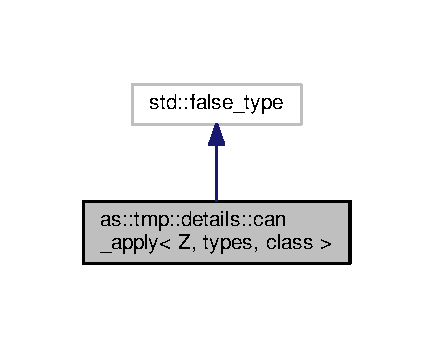
\includegraphics[width=208pt]{structas_1_1tmp_1_1details_1_1can__apply__inherit__graph}
\end{center}
\end{figure}


Collaboration diagram for as\+:\+:tmp\+:\+:details\+:\+:can\+\_\+apply$<$ Z, types, class $>$\+:
\nopagebreak
\begin{figure}[H]
\begin{center}
\leavevmode
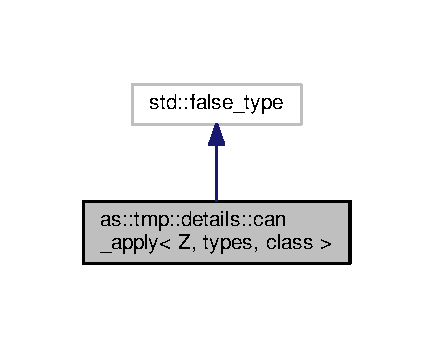
\includegraphics[width=208pt]{structas_1_1tmp_1_1details_1_1can__apply__coll__graph}
\end{center}
\end{figure}


The documentation for this struct was generated from the following file\+:\begin{DoxyCompactItemize}
\item 
src/\hyperlink{can__apply_8h}{can\+\_\+apply.\+h}\end{DoxyCompactItemize}

\hypertarget{structas_1_1tmp_1_1details_1_1can__apply_3_01Z_00_01types_3_01Ts_8_8_8_01_4_00_01std_1_1void__t_d0380c4f39b26cf3dcf2ed45500ba357}{}\section{as\+:\+:tmp\+:\+:details\+:\+:can\+\_\+apply$<$ Z, types$<$ Ts... $>$, std\+:\+:void\+\_\+t$<$ Z$<$ Ts... $>$ $>$ $>$ Struct Template Reference}
\label{structas_1_1tmp_1_1details_1_1can__apply_3_01Z_00_01types_3_01Ts_8_8_8_01_4_00_01std_1_1void__t_d0380c4f39b26cf3dcf2ed45500ba357}\index{as\+::tmp\+::details\+::can\+\_\+apply$<$ Z, types$<$ Ts... $>$, std\+::void\+\_\+t$<$ Z$<$ Ts... $>$ $>$ $>$@{as\+::tmp\+::details\+::can\+\_\+apply$<$ Z, types$<$ Ts... $>$, std\+::void\+\_\+t$<$ Z$<$ Ts... $>$ $>$ $>$}}


{\ttfamily \#include $<$can\+\_\+apply.\+h$>$}



Inheritance diagram for as\+:\+:tmp\+:\+:details\+:\+:can\+\_\+apply$<$ Z, types$<$ Ts... $>$, std\+:\+:void\+\_\+t$<$ Z$<$ Ts... $>$ $>$ $>$\+:
\nopagebreak
\begin{figure}[H]
\begin{center}
\leavevmode
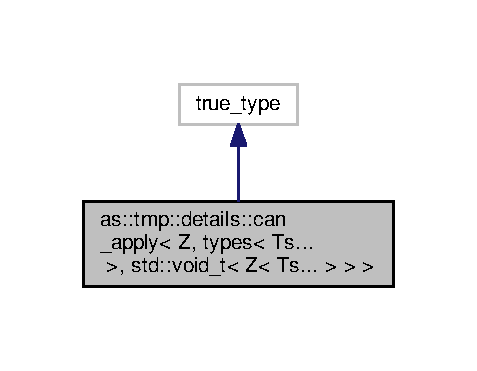
\includegraphics[width=229pt]{structas_1_1tmp_1_1details_1_1can__apply_3_01Z_00_01types_3_01Ts_8_8_8_01_4_00_01std_1_1void__t_299e711cbe14dcd24ae19586cb63c206}
\end{center}
\end{figure}


Collaboration diagram for as\+:\+:tmp\+:\+:details\+:\+:can\+\_\+apply$<$ Z, types$<$ Ts... $>$, std\+:\+:void\+\_\+t$<$ Z$<$ Ts... $>$ $>$ $>$\+:
\nopagebreak
\begin{figure}[H]
\begin{center}
\leavevmode
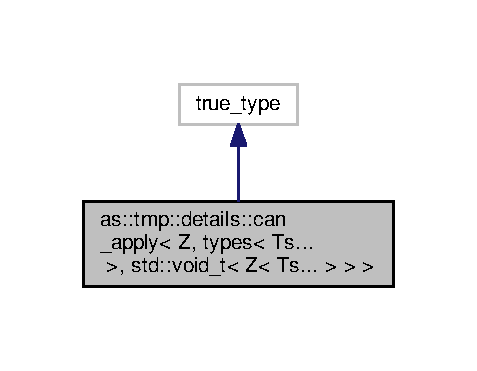
\includegraphics[width=229pt]{structas_1_1tmp_1_1details_1_1can__apply_3_01Z_00_01types_3_01Ts_8_8_8_01_4_00_01std_1_1void__t_5dee29e932352e51efcbc7ee5aec093f}
\end{center}
\end{figure}


The documentation for this struct was generated from the following file\+:\begin{DoxyCompactItemize}
\item 
src/\hyperlink{can__apply_8h}{can\+\_\+apply.\+h}\end{DoxyCompactItemize}

\hypertarget{structas_1_1tmp_1_1details_1_1is__associative}{}\section{as\+:\+:tmp\+:\+:details\+:\+:is\+\_\+associative$<$ class, class $>$ Struct Template Reference}
\label{structas_1_1tmp_1_1details_1_1is__associative}\index{as\+::tmp\+::details\+::is\+\_\+associative$<$ class, class $>$@{as\+::tmp\+::details\+::is\+\_\+associative$<$ class, class $>$}}


{\ttfamily \#include $<$is\+\_\+associative.\+h$>$}



Inheritance diagram for as\+:\+:tmp\+:\+:details\+:\+:is\+\_\+associative$<$ class, class $>$\+:
\nopagebreak
\begin{figure}[H]
\begin{center}
\leavevmode
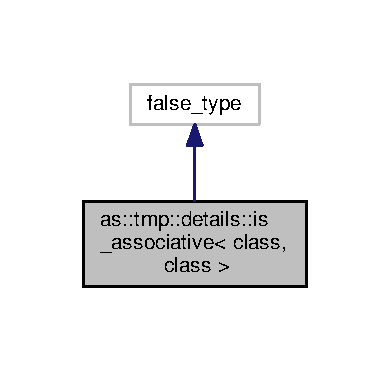
\includegraphics[width=187pt]{structas_1_1tmp_1_1details_1_1is__associative__inherit__graph}
\end{center}
\end{figure}


Collaboration diagram for as\+:\+:tmp\+:\+:details\+:\+:is\+\_\+associative$<$ class, class $>$\+:
\nopagebreak
\begin{figure}[H]
\begin{center}
\leavevmode
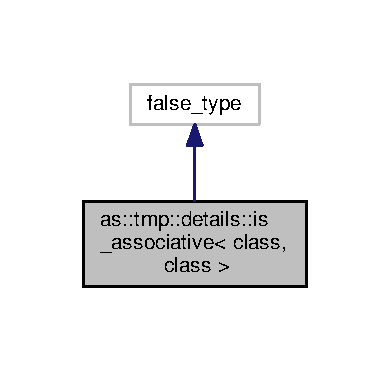
\includegraphics[width=187pt]{structas_1_1tmp_1_1details_1_1is__associative__coll__graph}
\end{center}
\end{figure}


The documentation for this struct was generated from the following file\+:\begin{DoxyCompactItemize}
\item 
src/\hyperlink{is__associative_8h}{is\+\_\+associative.\+h}\end{DoxyCompactItemize}

\hypertarget{structas_1_1tmp_1_1details_1_1is__associative_3_01Container_00_01std_1_1void__t_3_01typename_01Container_1_1key__type_01_4_01_4}{}\section{as\+:\+:tmp\+:\+:details\+:\+:is\+\_\+associative$<$ Container, std\+:\+:void\+\_\+t$<$ typename Container\+:\+:key\+\_\+type $>$ $>$ Struct Template Reference}
\label{structas_1_1tmp_1_1details_1_1is__associative_3_01Container_00_01std_1_1void__t_3_01typename_01Container_1_1key__type_01_4_01_4}\index{as\+::tmp\+::details\+::is\+\_\+associative$<$ Container, std\+::void\+\_\+t$<$ typename Container\+::key\+\_\+type $>$ $>$@{as\+::tmp\+::details\+::is\+\_\+associative$<$ Container, std\+::void\+\_\+t$<$ typename Container\+::key\+\_\+type $>$ $>$}}


{\ttfamily \#include $<$is\+\_\+associative.\+h$>$}



Inheritance diagram for as\+:\+:tmp\+:\+:details\+:\+:is\+\_\+associative$<$ Container, std\+:\+:void\+\_\+t$<$ typename Container\+:\+:key\+\_\+type $>$ $>$\+:\nopagebreak
\begin{figure}[H]
\begin{center}
\leavevmode
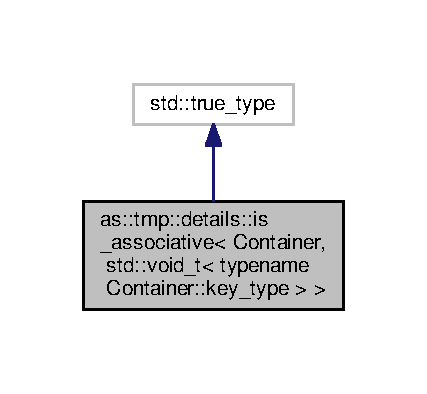
\includegraphics[width=205pt]{structas_1_1tmp_1_1details_1_1is__associative_3_01Container_00_01std_1_1void__t_3_01typename_01C611a54dcc77bf996638028d6bc5cb78d}
\end{center}
\end{figure}


Collaboration diagram for as\+:\+:tmp\+:\+:details\+:\+:is\+\_\+associative$<$ Container, std\+:\+:void\+\_\+t$<$ typename Container\+:\+:key\+\_\+type $>$ $>$\+:\nopagebreak
\begin{figure}[H]
\begin{center}
\leavevmode
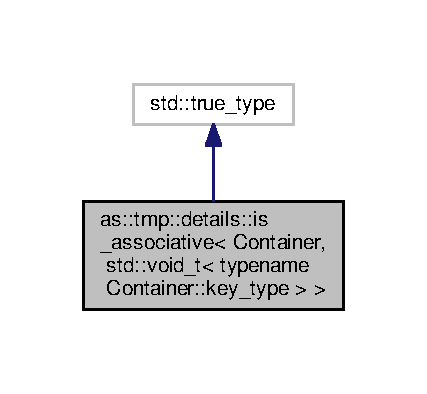
\includegraphics[width=205pt]{structas_1_1tmp_1_1details_1_1is__associative_3_01Container_00_01std_1_1void__t_3_01typename_01Caac0f829afd0b76a0bf08a7b10e9df26}
\end{center}
\end{figure}


The documentation for this struct was generated from the following file\+:\begin{DoxyCompactItemize}
\item 
src/\hyperlink{is__associative_8h}{is\+\_\+associative.\+h}\end{DoxyCompactItemize}

\hypertarget{classas_1_1iterator__pair}{}\section{as\+:\+:iterator\+\_\+pair$<$ Iterator $>$ Class Template Reference}
\label{classas_1_1iterator__pair}\index{as\+::iterator\+\_\+pair$<$ Iterator $>$@{as\+::iterator\+\_\+pair$<$ Iterator $>$}}


This class wraps a pair of begin and end iterators, and exposes them via \hyperlink{classas_1_1iterator__pair_a88c00afafd5ee4477b7ab2a1a89bb746}{begin()} and \hyperlink{classas_1_1iterator__pair_ae7cef6e91faecd20e6aebd2f21b29b41}{end()} function, which can be used in range-\/based for loops.  




{\ttfamily \#include $<$iterator\+\_\+pair.\+h$>$}

\subsection*{Public Member Functions}
\begin{DoxyCompactItemize}
\item 
\hyperlink{classas_1_1iterator__pair_a70030e7948493718b4baf500344a86e0}{iterator\+\_\+pair} (Iterator b, Iterator e)
\begin{DoxyCompactList}\small\item\em Constructor receiving the iterators. \end{DoxyCompactList}\item 
Iterator \hyperlink{classas_1_1iterator__pair_a88c00afafd5ee4477b7ab2a1a89bb746}{begin} () const
\begin{DoxyCompactList}\small\item\em Gives the begin iterator. \end{DoxyCompactList}\item 
Iterator \hyperlink{classas_1_1iterator__pair_ae7cef6e91faecd20e6aebd2f21b29b41}{end} () const
\begin{DoxyCompactList}\small\item\em Gives the end iterator. \end{DoxyCompactList}\end{DoxyCompactItemize}


\subsection{Detailed Description}
\subsubsection*{template$<$class Iterator$>$\newline
class as\+::iterator\+\_\+pair$<$ Iterator $>$}

This class wraps a pair of begin and end iterators, and exposes them via \hyperlink{classas_1_1iterator__pair_a88c00afafd5ee4477b7ab2a1a89bb746}{begin()} and \hyperlink{classas_1_1iterator__pair_ae7cef6e91faecd20e6aebd2f21b29b41}{end()} function, which can be used in range-\/based for loops. 


\begin{DoxyTemplParams}{Template Parameters}
{\em Iterator} & The iterator type. \\
\hline
\end{DoxyTemplParams}


\subsection{Constructor \& Destructor Documentation}
\mbox{\Hypertarget{classas_1_1iterator__pair_a70030e7948493718b4baf500344a86e0}\label{classas_1_1iterator__pair_a70030e7948493718b4baf500344a86e0}} 
\index{as\+::iterator\+\_\+pair@{as\+::iterator\+\_\+pair}!iterator\+\_\+pair@{iterator\+\_\+pair}}
\index{iterator\+\_\+pair@{iterator\+\_\+pair}!as\+::iterator\+\_\+pair@{as\+::iterator\+\_\+pair}}
\subsubsection{\texorpdfstring{iterator\+\_\+pair()}{iterator\_pair()}}
{\footnotesize\ttfamily template$<$class Iterator $>$ \\
\hyperlink{classas_1_1iterator__pair}{as\+::iterator\+\_\+pair}$<$ Iterator $>$\+::\hyperlink{classas_1_1iterator__pair}{iterator\+\_\+pair} (\begin{DoxyParamCaption}\item[{Iterator}]{b,  }\item[{Iterator}]{e }\end{DoxyParamCaption})\hspace{0.3cm}{\ttfamily [inline]}}



Constructor receiving the iterators. 


\begin{DoxyParams}{Parameters}
{\em b} & Begin iterator. \\
\hline
{\em e} & End iterator. \\
\hline
\end{DoxyParams}


\subsection{Member Function Documentation}
\mbox{\Hypertarget{classas_1_1iterator__pair_a88c00afafd5ee4477b7ab2a1a89bb746}\label{classas_1_1iterator__pair_a88c00afafd5ee4477b7ab2a1a89bb746}} 
\index{as\+::iterator\+\_\+pair@{as\+::iterator\+\_\+pair}!begin@{begin}}
\index{begin@{begin}!as\+::iterator\+\_\+pair@{as\+::iterator\+\_\+pair}}
\subsubsection{\texorpdfstring{begin()}{begin()}}
{\footnotesize\ttfamily template$<$class Iterator $>$ \\
Iterator \hyperlink{classas_1_1iterator__pair}{as\+::iterator\+\_\+pair}$<$ Iterator $>$\+::begin (\begin{DoxyParamCaption}{ }\end{DoxyParamCaption}) const\hspace{0.3cm}{\ttfamily [inline]}}



Gives the begin iterator. 

\begin{DoxyReturn}{Returns}
The begin iterator. 
\end{DoxyReturn}
\mbox{\Hypertarget{classas_1_1iterator__pair_ae7cef6e91faecd20e6aebd2f21b29b41}\label{classas_1_1iterator__pair_ae7cef6e91faecd20e6aebd2f21b29b41}} 
\index{as\+::iterator\+\_\+pair@{as\+::iterator\+\_\+pair}!end@{end}}
\index{end@{end}!as\+::iterator\+\_\+pair@{as\+::iterator\+\_\+pair}}
\subsubsection{\texorpdfstring{end()}{end()}}
{\footnotesize\ttfamily template$<$class Iterator $>$ \\
Iterator \hyperlink{classas_1_1iterator__pair}{as\+::iterator\+\_\+pair}$<$ Iterator $>$\+::end (\begin{DoxyParamCaption}{ }\end{DoxyParamCaption}) const\hspace{0.3cm}{\ttfamily [inline]}}



Gives the end iterator. 

\begin{DoxyReturn}{Returns}
The end iterator. 
\end{DoxyReturn}


The documentation for this class was generated from the following file\+:\begin{DoxyCompactItemize}
\item 
src/\hyperlink{iterator__pair_8h}{iterator\+\_\+pair.\+h}\end{DoxyCompactItemize}

\hypertarget{structas_1_1tmp_1_1types}{}\section{as\+:\+:tmp\+:\+:types$<$... $>$ Struct Template Reference}
\label{structas_1_1tmp_1_1types}\index{as\+::tmp\+::types$<$... $>$@{as\+::tmp\+::types$<$... $>$}}


{\ttfamily \#include $<$can\+\_\+apply.\+h$>$}

\subsection*{Public Types}
\begin{DoxyCompactItemize}
\item 
using \hyperlink{structas_1_1tmp_1_1types_a8fee0852270845709fbb995347ac8fa3}{type} = \hyperlink{structas_1_1tmp_1_1types}{types}
\end{DoxyCompactItemize}


\subsection{Member Typedef Documentation}
\mbox{\Hypertarget{structas_1_1tmp_1_1types_a8fee0852270845709fbb995347ac8fa3}\label{structas_1_1tmp_1_1types_a8fee0852270845709fbb995347ac8fa3}} 
\index{as\+::tmp\+::types@{as\+::tmp\+::types}!type@{type}}
\index{type@{type}!as\+::tmp\+::types@{as\+::tmp\+::types}}
\subsubsection{\texorpdfstring{type}{type}}
{\footnotesize\ttfamily template$<$class... $>$ \\
using \hyperlink{structas_1_1tmp_1_1types}{as\+::tmp\+::types}$<$... $>$\+::\hyperlink{structas_1_1tmp_1_1types_a8fee0852270845709fbb995347ac8fa3}{type} =  \hyperlink{structas_1_1tmp_1_1types}{types}}



The documentation for this struct was generated from the following file\+:\begin{DoxyCompactItemize}
\item 
src/\hyperlink{can__apply_8h}{can\+\_\+apply.\+h}\end{DoxyCompactItemize}

\chapter{File Documentation}
\hypertarget{and__die_8h}{}\section{src/and\+\_\+die.h File Reference}
\label{and__die_8h}\index{src/and\+\_\+die.\+h@{src/and\+\_\+die.\+h}}
{\ttfamily \#include $<$ostream$>$}\newline
{\ttfamily \#include $<$cstdlib$>$}\newline
Include dependency graph for and\+\_\+die.\+h\+:\nopagebreak
\begin{figure}[H]
\begin{center}
\leavevmode
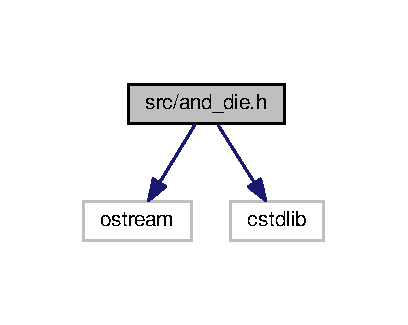
\includegraphics[width=196pt]{and__die_8h__incl}
\end{center}
\end{figure}
\subsection*{Classes}
\begin{DoxyCompactItemize}
\item 
struct \hyperlink{structas_1_1and__die}{as\+::and\+\_\+die}
\begin{DoxyCompactList}\small\item\em A struct used to signal that the programme should be terminated immediately (die). \end{DoxyCompactList}\end{DoxyCompactItemize}
\subsection*{Namespaces}
\begin{DoxyCompactItemize}
\item 
 \hyperlink{namespaceas}{as}
\end{DoxyCompactItemize}
\subsection*{Functions}
\begin{DoxyCompactItemize}
\item 
std\+::ostream \& \hyperlink{namespaceas_a4d891ae352512e1c506d6cd01ff1422c}{as\+::operator$<$$<$} (std\+::ostream \&out, const and\+\_\+die \&)
\begin{DoxyCompactList}\small\item\em Concatenates a \hyperlink{structas_1_1and__die}{and\+\_\+die} structure to an output stream, to immediately terminate a programme. \end{DoxyCompactList}\end{DoxyCompactItemize}

\hypertarget{as__version_8h}{}\section{src/as\+\_\+version.h File Reference}
\label{as__version_8h}\index{src/as\+\_\+version.\+h@{src/as\+\_\+version.\+h}}


Keeps track of the as library major, minor, and build version numbers.  


\subsection*{Macros}
\begin{DoxyCompactItemize}
\item 
\#define \hyperlink{as__version_8h_a4655bc98bf611ce7a8a37250ad8cc943}{A\+S\+\_\+\+V\+E\+R\+S\+I\+O\+N\+\_\+\+M\+A\+J\+OR}~0
\begin{DoxyCompactList}\small\item\em Major version of the as library. \end{DoxyCompactList}\item 
\#define \hyperlink{as__version_8h_ac016426c7e016d0c3673cbbcc3db3083}{A\+S\+\_\+\+V\+E\+R\+S\+I\+O\+N\+\_\+\+M\+I\+N\+OR}~0
\begin{DoxyCompactList}\small\item\em Minor version of the as library. \end{DoxyCompactList}\item 
\#define \hyperlink{as__version_8h_a6a52de62e56ab76f01f20e546c97240f}{A\+S\+\_\+\+V\+E\+R\+S\+I\+O\+N\+\_\+\+B\+U\+I\+LD}~1
\begin{DoxyCompactList}\small\item\em Build version of the as library. \end{DoxyCompactList}\end{DoxyCompactItemize}


\subsection{Detailed Description}
Keeps track of the as library major, minor, and build version numbers. 



\subsection{Macro Definition Documentation}
\mbox{\Hypertarget{as__version_8h_a6a52de62e56ab76f01f20e546c97240f}\label{as__version_8h_a6a52de62e56ab76f01f20e546c97240f}} 
\index{as\+\_\+version.\+h@{as\+\_\+version.\+h}!A\+S\+\_\+\+V\+E\+R\+S\+I\+O\+N\+\_\+\+B\+U\+I\+LD@{A\+S\+\_\+\+V\+E\+R\+S\+I\+O\+N\+\_\+\+B\+U\+I\+LD}}
\index{A\+S\+\_\+\+V\+E\+R\+S\+I\+O\+N\+\_\+\+B\+U\+I\+LD@{A\+S\+\_\+\+V\+E\+R\+S\+I\+O\+N\+\_\+\+B\+U\+I\+LD}!as\+\_\+version.\+h@{as\+\_\+version.\+h}}
\subsubsection{\texorpdfstring{A\+S\+\_\+\+V\+E\+R\+S\+I\+O\+N\+\_\+\+B\+U\+I\+LD}{AS\_VERSION\_BUILD}}
{\footnotesize\ttfamily \#define A\+S\+\_\+\+V\+E\+R\+S\+I\+O\+N\+\_\+\+B\+U\+I\+LD~1}



Build version of the as library. 

\mbox{\Hypertarget{as__version_8h_a4655bc98bf611ce7a8a37250ad8cc943}\label{as__version_8h_a4655bc98bf611ce7a8a37250ad8cc943}} 
\index{as\+\_\+version.\+h@{as\+\_\+version.\+h}!A\+S\+\_\+\+V\+E\+R\+S\+I\+O\+N\+\_\+\+M\+A\+J\+OR@{A\+S\+\_\+\+V\+E\+R\+S\+I\+O\+N\+\_\+\+M\+A\+J\+OR}}
\index{A\+S\+\_\+\+V\+E\+R\+S\+I\+O\+N\+\_\+\+M\+A\+J\+OR@{A\+S\+\_\+\+V\+E\+R\+S\+I\+O\+N\+\_\+\+M\+A\+J\+OR}!as\+\_\+version.\+h@{as\+\_\+version.\+h}}
\subsubsection{\texorpdfstring{A\+S\+\_\+\+V\+E\+R\+S\+I\+O\+N\+\_\+\+M\+A\+J\+OR}{AS\_VERSION\_MAJOR}}
{\footnotesize\ttfamily \#define A\+S\+\_\+\+V\+E\+R\+S\+I\+O\+N\+\_\+\+M\+A\+J\+OR~0}



Major version of the as library. 

\mbox{\Hypertarget{as__version_8h_ac016426c7e016d0c3673cbbcc3db3083}\label{as__version_8h_ac016426c7e016d0c3673cbbcc3db3083}} 
\index{as\+\_\+version.\+h@{as\+\_\+version.\+h}!A\+S\+\_\+\+V\+E\+R\+S\+I\+O\+N\+\_\+\+M\+I\+N\+OR@{A\+S\+\_\+\+V\+E\+R\+S\+I\+O\+N\+\_\+\+M\+I\+N\+OR}}
\index{A\+S\+\_\+\+V\+E\+R\+S\+I\+O\+N\+\_\+\+M\+I\+N\+OR@{A\+S\+\_\+\+V\+E\+R\+S\+I\+O\+N\+\_\+\+M\+I\+N\+OR}!as\+\_\+version.\+h@{as\+\_\+version.\+h}}
\subsubsection{\texorpdfstring{A\+S\+\_\+\+V\+E\+R\+S\+I\+O\+N\+\_\+\+M\+I\+N\+OR}{AS\_VERSION\_MINOR}}
{\footnotesize\ttfamily \#define A\+S\+\_\+\+V\+E\+R\+S\+I\+O\+N\+\_\+\+M\+I\+N\+OR~0}



Minor version of the as library. 


\hypertarget{can__apply_8h}{}\section{src/can\+\_\+apply.h File Reference}
\label{can__apply_8h}\index{src/can\+\_\+apply.\+h@{src/can\+\_\+apply.\+h}}
{\ttfamily \#include $<$type\+\_\+traits$>$}\newline
Include dependency graph for can\+\_\+apply.\+h\+:
\nopagebreak
\begin{figure}[H]
\begin{center}
\leavevmode
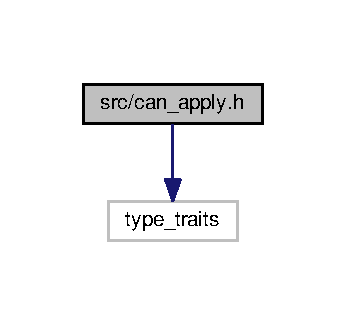
\includegraphics[width=166pt]{can__apply_8h__incl}
\end{center}
\end{figure}
This graph shows which files directly or indirectly include this file\+:
\nopagebreak
\begin{figure}[H]
\begin{center}
\leavevmode
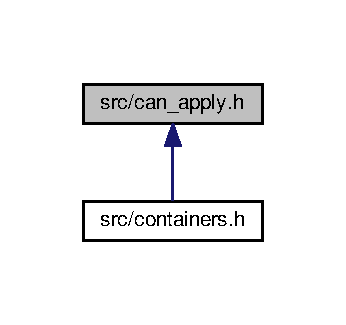
\includegraphics[width=166pt]{can__apply_8h__dep__incl}
\end{center}
\end{figure}
\subsection*{Classes}
\begin{DoxyCompactItemize}
\item 
struct \hyperlink{structas_1_1tmp_1_1types}{as\+::tmp\+::types$<$... $>$}
\item 
struct \hyperlink{structas_1_1tmp_1_1details_1_1can__apply}{as\+::tmp\+::details\+::can\+\_\+apply$<$ Z, types, class $>$}
\item 
struct \hyperlink{structas_1_1tmp_1_1details_1_1can__apply_3_01Z_00_01types_3_01Ts_8_8_8_01_4_00_01std_1_1void__t_d0380c4f39b26cf3dcf2ed45500ba357}{as\+::tmp\+::details\+::can\+\_\+apply$<$ Z, types$<$ Ts... $>$, std\+::void\+\_\+t$<$ Z$<$ Ts... $>$ $>$ $>$}
\end{DoxyCompactItemize}
\subsection*{Namespaces}
\begin{DoxyCompactItemize}
\item 
 \hyperlink{namespaceas}{as}
\item 
 \hyperlink{namespacetmp}{tmp}
\begin{DoxyCompactList}\small\item\em Template-\/meta-\/programming namespace. \end{DoxyCompactList}\item 
 \hyperlink{namespaceas_1_1tmp}{as\+::tmp}
\item 
 \hyperlink{namespaceas_1_1tmp_1_1details}{as\+::tmp\+::details}
\end{DoxyCompactItemize}
\subsection*{Typedefs}
\begin{DoxyCompactItemize}
\item 
{\footnotesize template$<$template$<$ class... $>$ class Z, class... Ts$>$ }\\using \hyperlink{namespaceas_1_1tmp_a44a275bd3c66d727fb1b6f0179d49e19}{as\+::tmp\+::can\+\_\+apply} = details\+::can\+\_\+apply$<$ Z, types$<$ Ts... $>$ $>$
\begin{DoxyCompactList}\small\item\em Checks if the application of arguments to a templated class is valid. \end{DoxyCompactList}\end{DoxyCompactItemize}

\hypertarget{console_8h}{}\section{src/console.h File Reference}
\label{console_8h}\index{src/console.\+h@{src/console.\+h}}
{\ttfamily \#include $<$string$>$}\newline
{\ttfamily \#include $<$ostream$>$}\newline
{\ttfamily \#include $<$type\+\_\+traits$>$}\newline
{\ttfamily \#include $<$sstream$>$}\newline
Include dependency graph for console.\+h\+:\nopagebreak
\begin{figure}[H]
\begin{center}
\leavevmode
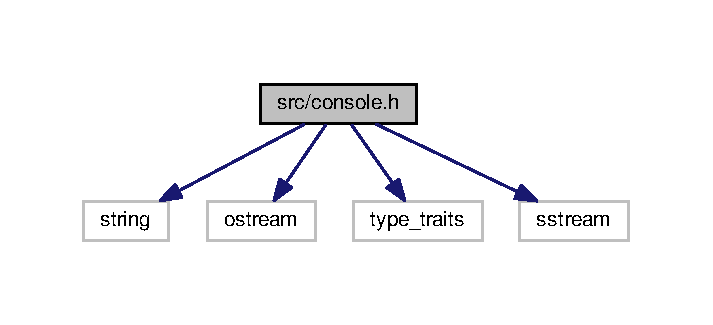
\includegraphics[width=342pt]{console_8h__incl}
\end{center}
\end{figure}
This graph shows which files directly or indirectly include this file\+:\nopagebreak
\begin{figure}[H]
\begin{center}
\leavevmode
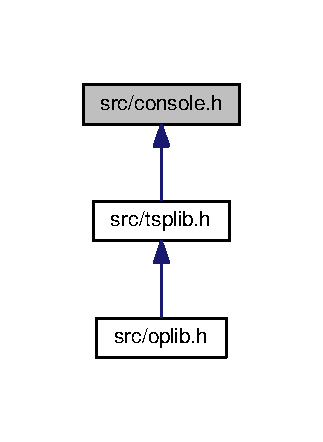
\includegraphics[width=155pt]{console_8h__dep__incl}
\end{center}
\end{figure}
\subsection*{Namespaces}
\begin{DoxyCompactItemize}
\item 
 \hyperlink{namespaceas}{as}
\item 
 \hyperlink{namespaceconsole}{console}
\begin{DoxyCompactList}\small\item\em This namespace contains miscellaneous console utilities. \end{DoxyCompactList}\item 
 \hyperlink{namespaceas_1_1console}{as\+::console}
\end{DoxyCompactItemize}
\subsection*{Enumerations}
\begin{DoxyCompactItemize}
\item 
enum \hyperlink{namespaceas_1_1console_ab2f5a531e43f4ee9e0f348f8aa5ce16c}{as\+::console\+::\+Colour} \{ \newline
\hyperlink{namespaceas_1_1console_ab2f5a531e43f4ee9e0f348f8aa5ce16caee38e4d5dd68c4e440825018d549cb47}{as\+::console\+::\+Colour\+::\+Red} = 31, 
\hyperlink{namespaceas_1_1console_ab2f5a531e43f4ee9e0f348f8aa5ce16cad382816a3cbeed082c9e216e7392eed1}{as\+::console\+::\+Colour\+::\+Green} = 32, 
\hyperlink{namespaceas_1_1console_ab2f5a531e43f4ee9e0f348f8aa5ce16ca51e6cd92b6c45f9affdc158ecca2b8b8}{as\+::console\+::\+Colour\+::\+Yellow} = 33, 
\hyperlink{namespaceas_1_1console_ab2f5a531e43f4ee9e0f348f8aa5ce16ca9594eec95be70e7b1710f730fdda33d9}{as\+::console\+::\+Colour\+::\+Blue} = 34, 
\newline
\hyperlink{namespaceas_1_1console_ab2f5a531e43f4ee9e0f348f8aa5ce16cab91cc2c1416fcca942b61c7ac5b1a9ac}{as\+::console\+::\+Colour\+::\+Magenta} = 35, 
\hyperlink{namespaceas_1_1console_ab2f5a531e43f4ee9e0f348f8aa5ce16ca7a1920d61156abc05a60135aefe8bc67}{as\+::console\+::\+Colour\+::\+Default} = 39
 \}\begin{DoxyCompactList}\small\item\em Console colour codes. \end{DoxyCompactList}
\end{DoxyCompactItemize}
\subsection*{Functions}
\begin{DoxyCompactItemize}
\item 
constexpr std\+::underlying\+\_\+type$<$ Colour $>$\+::type \hyperlink{namespaceas_1_1console_ae7e08b7053b857ff4d798c9860680ac7}{as\+::console\+::colour\+\_\+code} (const Colour \&c)
\begin{DoxyCompactList}\small\item\em Gives the numerical code corresponding to the colour. \end{DoxyCompactList}\item 
std\+::string \hyperlink{namespaceas_1_1console_a960fbc86f1ff964059acb44b12342199}{as\+::console\+::escape} (Colour c)
\begin{DoxyCompactList}\small\item\em Gives a string with the escape codes relative to the colour. \end{DoxyCompactList}\item 
std\+::ostream \& \hyperlink{namespaceas_1_1console_a05dafe6fcc36510443d4769ad4667652}{as\+::console\+::operator$<$$<$} (std\+::ostream \&out, const Colour \&c)
\begin{DoxyCompactList}\small\item\em Prints a colour code. \end{DoxyCompactList}\item 
{\footnotesize template$<$class T $>$ }\\std\+::string \hyperlink{namespaceas_1_1console_a64c8640b4ced55636cb8926b1640d6e9}{as\+::console\+::colourise} (Colour c, const T \&what)
\begin{DoxyCompactList}\small\item\em Colours some content and then resets the colour to default. \end{DoxyCompactList}\end{DoxyCompactItemize}

\hypertarget{containers_8h}{}\section{src/containers.h File Reference}
\label{containers_8h}\index{src/containers.\+h@{src/containers.\+h}}
{\ttfamily \#include \char`\"{}can\+\_\+apply.\+h\char`\"{}}\newline
{\ttfamily \#include \char`\"{}is\+\_\+associative.\+h\char`\"{}}\newline
{\ttfamily \#include $<$algorithm$>$}\newline
{\ttfamily \#include $<$set$>$}\newline
{\ttfamily \#include $<$iostream$>$}\newline
Include dependency graph for containers.\+h\+:
\nopagebreak
\begin{figure}[H]
\begin{center}
\leavevmode
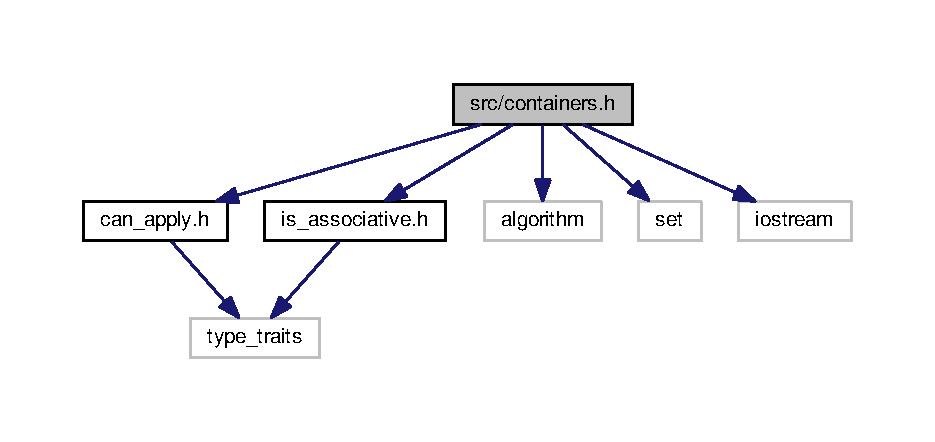
\includegraphics[width=350pt]{containers_8h__incl}
\end{center}
\end{figure}
\subsection*{Namespaces}
\begin{DoxyCompactItemize}
\item 
 \hyperlink{namespaceas}{as}
\item 
 \hyperlink{namespaceas_1_1details}{as\+::details}
\end{DoxyCompactItemize}
\subsection*{Typedefs}
\begin{DoxyCompactItemize}
\item 
{\footnotesize template$<$class Container , class T $>$ }\\using \hyperlink{namespaceas_a9bd788709567003423247a9db4ba1074}{as\+::count\+\_\+method\+\_\+type} = decltype(std\+::declval$<$ Container $>$().count(std\+::declval$<$ T $>$()))
\begin{DoxyCompactList}\small\item\em This is the type of a generic .count() method for a container. \end{DoxyCompactList}\item 
{\footnotesize template$<$class Container , class T $>$ }\\using \hyperlink{namespaceas_a9e0fcaa3ddb46647d8979282465685da}{as\+::has\+\_\+count\+\_\+method} = tmp\+::can\+\_\+apply$<$ count\+\_\+method\+\_\+type, Container, T $>$
\begin{DoxyCompactList}\small\item\em This will inherit from true\+\_\+type iff class Container has an appopriate .count() method. \end{DoxyCompactList}\end{DoxyCompactItemize}
\subsection*{Functions}
\begin{DoxyCompactItemize}
\item 
{\footnotesize template$<$class Container , class T $>$ }\\bool \hyperlink{namespaceas_1_1details_aaa1e2c1c370bddd0020956d333bbef26}{as\+::details\+::contains} (std\+::false\+\_\+type, const Container \&container, const T \&element)
\item 
{\footnotesize template$<$class Container , class T $>$ }\\bool \hyperlink{namespaceas_1_1details_aa25b4a9ab19e3b807bbd58dc208d2607}{as\+::details\+::contains} (std\+::true\+\_\+type, const Container \&container, const T \&element)
\item 
{\footnotesize template$<$class Container , class T $>$ }\\bool \hyperlink{namespaceas_a49cf7ae4239ab51e54f099d30a84811a}{as\+::contains} (const Container \&container, const T \&element)
\begin{DoxyCompactList}\small\item\em Tells whether a container contains a certain element. \end{DoxyCompactList}\item 
{\footnotesize template$<$class Value $>$ }\\std\+::ostream \& \hyperlink{namespaceas_1_1details_a2e51ab78c6720ab244aa4cd08c5e7b55}{as\+::details\+::iterated\+\_\+value} (const Value \&value, std\+::ostream \&out)
\item 
{\footnotesize template$<$class Key , class Value $>$ }\\std\+::ostream \& \hyperlink{namespaceas_1_1details_abb914e2826b38ed8ae4d2f8004843689}{as\+::details\+::iterated\+\_\+value} (const std\+::pair$<$ Key, Value $>$ \&key\+\_\+val, std\+::ostream \&out)
\item 
{\footnotesize template$<$class Container $>$ }\\void \hyperlink{namespaceas_aab6569c28591bebed9bd29b40c772bfc}{as\+::join\+\_\+and\+\_\+print} (const Container \&container, std\+::ostream \&out=std\+::cout, std\+::string separator=\char`\"{}, \char`\"{})
\begin{DoxyCompactList}\small\item\em Joins the elements of a container using the separator, and prints the result to an output stream. \end{DoxyCompactList}\end{DoxyCompactItemize}

\hypertarget{file__stream_8h}{}\section{src/file\+\_\+stream.h File Reference}
\label{file__stream_8h}\index{src/file\+\_\+stream.\+h@{src/file\+\_\+stream.\+h}}
{\ttfamily \#include $<$cstddef$>$}\newline
{\ttfamily \#include $<$fstream$>$}\newline
{\ttfamily \#include $<$limits$>$}\newline
Include dependency graph for file\+\_\+stream.\+h\+:\nopagebreak
\begin{figure}[H]
\begin{center}
\leavevmode
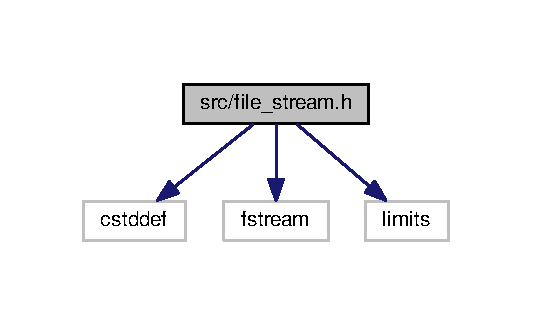
\includegraphics[width=256pt]{file__stream_8h__incl}
\end{center}
\end{figure}
\subsection*{Namespaces}
\begin{DoxyCompactItemize}
\item 
 \hyperlink{namespaceas}{as}
\end{DoxyCompactItemize}
\subsection*{Functions}
\begin{DoxyCompactItemize}
\item 
void \hyperlink{namespaceas_a359f2d209e5ec052ec0d2752a589802d}{as\+::skip\+\_\+lines} (std\+::ifstream \&stream, std\+::size\+\_\+t how\+\_\+many=1u)
\begin{DoxyCompactList}\small\item\em Skips a certain number of lines from an input file stream. \end{DoxyCompactList}\end{DoxyCompactItemize}

\hypertarget{graph_8h}{}\section{src/graph.h File Reference}
\label{graph_8h}\index{src/graph.\+h@{src/graph.\+h}}
{\ttfamily \#include \char`\"{}iterator\+\_\+pair.\+h\char`\"{}}\newline
{\ttfamily \#include $<$boost/graph/graph\+\_\+traits.\+hpp$>$}\newline
{\ttfamily \#include $<$boost/graph/adjacency\+\_\+list.\+hpp$>$}\newline
Include dependency graph for graph.\+h\+:
\nopagebreak
\begin{figure}[H]
\begin{center}
\leavevmode
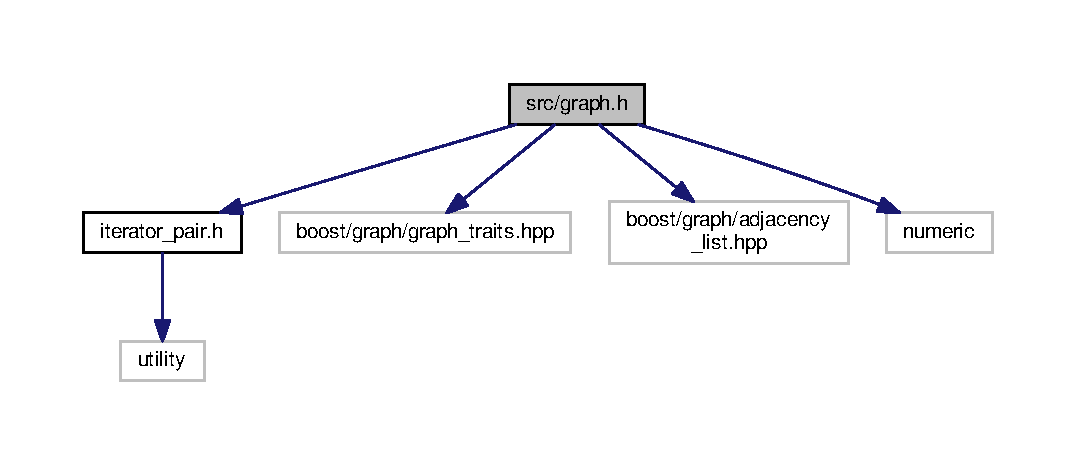
\includegraphics[width=350pt]{graph_8h__incl}
\end{center}
\end{figure}
\subsection*{Namespaces}
\begin{DoxyCompactItemize}
\item 
 \hyperlink{namespaceas}{as}
\item 
 \hyperlink{namespacegraph}{graph}
\begin{DoxyCompactList}\small\item\em This namespace provides functions which work with boost graphs. \end{DoxyCompactList}\item 
 \hyperlink{namespaceas_1_1graph}{as\+::graph}
\end{DoxyCompactItemize}
\subsection*{Functions}
\begin{DoxyCompactItemize}
\item 
{\footnotesize template$<$class Boost\+Graph $>$ }\\iterator\+\_\+pair$<$ typename boost\+::graph\+\_\+traits$<$ Boost\+Graph $>$\+::vertex\+\_\+iterator $>$ \hyperlink{namespaceas_1_1graph_ab93ee208eb116d3a3349c8de8cc91445}{as\+::graph\+::vertices} (const Boost\+Graph \&graph)
\begin{DoxyCompactList}\small\item\em Gives an \hyperlink{classas_1_1iterator__pair}{iterator\+\_\+pair} that can be used in range-\/based for loops to cycle through the vertices of a graph. \end{DoxyCompactList}\item 
{\footnotesize template$<$class Boost\+Graph $>$ }\\iterator\+\_\+pair$<$ typename boost\+::graph\+\_\+traits$<$ Boost\+Graph $>$\+::edge\+\_\+iterator $>$ \hyperlink{namespaceas_1_1graph_ae44b728c4acaf47bc2bb010831df9452}{as\+::graph\+::edges} (const Boost\+Graph \&graph)
\begin{DoxyCompactList}\small\item\em Gives an \hyperlink{classas_1_1iterator__pair}{iterator\+\_\+pair} that can be used in range-\/based for loops to cycle through the edges of a graph. \end{DoxyCompactList}\item 
{\footnotesize template$<$class Boost\+Graph $>$ }\\iterator\+\_\+pair$<$ typename boost\+::graph\+\_\+traits$<$ Boost\+Graph $>$\+::out\+\_\+edge\+\_\+iterator $>$ \hyperlink{namespaceas_1_1graph_a00143e178e97f0e9787802953d74a9f7}{as\+::graph\+::out\+\_\+edges} (const typename boost\+::graph\+\_\+traits$<$ Boost\+Graph $>$\+::vertex\+\_\+descriptor \&vertex, const Boost\+Graph \&graph)
\begin{DoxyCompactList}\small\item\em Gives an \hyperlink{classas_1_1iterator__pair}{iterator\+\_\+pair} that can be used in range-\/based for loops to cycle through the out-\/edges of a vertex of a graph. \end{DoxyCompactList}\item 
{\footnotesize template$<$class Boost\+Graph $>$ }\\iterator\+\_\+pair$<$ typename boost\+::graph\+\_\+traits$<$ Boost\+Graph $>$\+::in\+\_\+edge\+\_\+iterator $>$ \hyperlink{namespaceas_1_1graph_ab75a465b1d5869f0ea8b698f02b067aa}{as\+::graph\+::in\+\_\+edges} (const typename boost\+::graph\+\_\+traits$<$ Boost\+Graph $>$\+::vertex\+\_\+descriptor \&vertex, const Boost\+Graph \&graph)
\begin{DoxyCompactList}\small\item\em Gives an \hyperlink{classas_1_1iterator__pair}{iterator\+\_\+pair} that can be used in range-\/based for loops to cycle through the in-\/edges of a vertex of a graph. \end{DoxyCompactList}\item 
{\footnotesize template$<$class Boost\+Graph $>$ }\\iterator\+\_\+pair$<$ typename boost\+::graph\+\_\+traits$<$ Boost\+Graph $>$\+::adjacency\+\_\+iterator $>$ \hyperlink{namespaceas_1_1graph_a7a86ebb168cf6ac390a5bd86d3380350}{as\+::graph\+::neighbours} (const typename boost\+::graph\+\_\+traits$<$ Boost\+Graph $>$\+::vertex\+\_\+descriptor \&vertex, const Boost\+Graph \&graph)
\begin{DoxyCompactList}\small\item\em Gives an \hyperlink{classas_1_1iterator__pair}{iterator\+\_\+pair} that can be used in range-\/based for loops to cycle through the vertices adjacent to a given vertex, in an undirected graph. \end{DoxyCompactList}\item 
{\footnotesize template$<$class Boost\+Graph $>$ }\\bool \hyperlink{namespaceas_1_1graph_ac0b52ec1e242ac547157a42aac39e21a}{as\+::graph\+::incident\+\_\+to\+\_\+the\+\_\+same\+\_\+vertex} (const typename boost\+::graph\+\_\+traits$<$ Boost\+Graph $>$\+::edge\+\_\+descriptor \&edge1, const typename boost\+::graph\+\_\+traits$<$ Boost\+Graph $>$\+::edge\+\_\+descriptor \&edge2, const Boost\+Graph \&graph)
\begin{DoxyCompactList}\small\item\em Tells whether two edges of an undirected graph are incident to at least one common vertex. \end{DoxyCompactList}\item 
{\footnotesize template$<$class Boost\+Graph $>$ }\\bool \hyperlink{namespaceas_1_1graph_af020abed3b5b57f984d8ce940ee6f4cd}{as\+::graph\+::is\+\_\+extreme} (const typename boost\+::graph\+\_\+traits$<$ Boost\+Graph $>$\+::vertex\+\_\+descriptor \&vertex, const typename boost\+::graph\+\_\+traits$<$ Boost\+Graph $>$\+::edge\+\_\+descriptor \&edge, const Boost\+Graph \&graph)
\begin{DoxyCompactList}\small\item\em Tells whether a vertex is an extreme of an edge, i.\+e. if it is either its source or its target. For an undirected graph, therefore, it tells whether the edge is incident to the vertex. \end{DoxyCompactList}\item 
{\footnotesize template$<$class Boost\+Graph $>$ }\\boost\+::graph\+\_\+traits$<$ Boost\+Graph $>$\+::vertex\+\_\+descriptor \hyperlink{namespaceas_1_1graph_a592c192d63c1c42820da78708adb9e61}{as\+::graph\+::other\+\_\+extreme} (const typename boost\+::graph\+\_\+traits$<$ Boost\+Graph $>$\+::vertex\+\_\+descriptor \&vertex, const typename boost\+::graph\+\_\+traits$<$ Boost\+Graph $>$\+::edge\+\_\+descriptor \&edge, const Boost\+Graph \&graph)
\begin{DoxyCompactList}\small\item\em Given an edge and a vertex which is one of the two extremes of the edge, it returns the other extreme. \end{DoxyCompactList}\end{DoxyCompactItemize}

\hypertarget{is__associative_8h}{}\section{src/is\+\_\+associative.h File Reference}
\label{is__associative_8h}\index{src/is\+\_\+associative.\+h@{src/is\+\_\+associative.\+h}}
{\ttfamily \#include $<$type\+\_\+traits$>$}\newline
Include dependency graph for is\+\_\+associative.\+h\+:\nopagebreak
\begin{figure}[H]
\begin{center}
\leavevmode
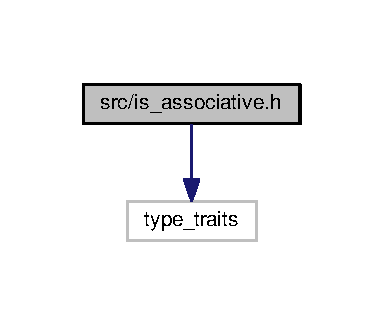
\includegraphics[width=184pt]{is__associative_8h__incl}
\end{center}
\end{figure}
This graph shows which files directly or indirectly include this file\+:\nopagebreak
\begin{figure}[H]
\begin{center}
\leavevmode
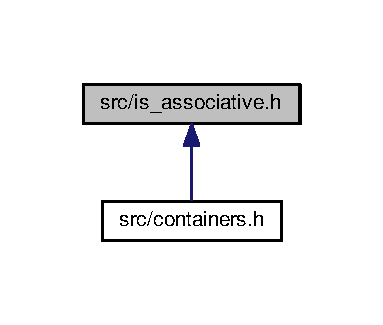
\includegraphics[width=184pt]{is__associative_8h__dep__incl}
\end{center}
\end{figure}
\subsection*{Classes}
\begin{DoxyCompactItemize}
\item 
struct \hyperlink{structas_1_1tmp_1_1details_1_1is__associative}{as\+::tmp\+::details\+::is\+\_\+associative$<$ class, class $>$}
\item 
struct \hyperlink{structas_1_1tmp_1_1details_1_1is__associative_3_01Container_00_01std_1_1void__t_3_01typename_01Container_1_1key__type_01_4_01_4}{as\+::tmp\+::details\+::is\+\_\+associative$<$ Container, std\+::void\+\_\+t$<$ typename Container\+::key\+\_\+type $>$ $>$}
\end{DoxyCompactItemize}
\subsection*{Namespaces}
\begin{DoxyCompactItemize}
\item 
 \hyperlink{namespaceas}{as}
\item 
 \hyperlink{namespacetmp}{tmp}
\begin{DoxyCompactList}\small\item\em Template-\/meta-\/programming namespace. \end{DoxyCompactList}\item 
 \hyperlink{namespaceas_1_1tmp}{as\+::tmp}
\item 
 \hyperlink{namespaceas_1_1tmp_1_1details}{as\+::tmp\+::details}
\end{DoxyCompactItemize}
\subsection*{Typedefs}
\begin{DoxyCompactItemize}
\item 
{\footnotesize template$<$class Container $>$ }\\using \hyperlink{namespaceas_1_1tmp_a893659f8b2cd22837c8f494a6f4a61d9}{as\+::tmp\+::is\+\_\+associative} = details\+::is\+\_\+associative$<$ Container $>$
\begin{DoxyCompactList}\small\item\em This type will be true\+\_\+type if the container is associative (i.\+e. it has a member type \char`\"{}key\+\_\+type\char`\"{}) or false\+\_\+type otherwise. \end{DoxyCompactList}\end{DoxyCompactItemize}

\hypertarget{iterator__pair_8h}{}\section{src/iterator\+\_\+pair.h File Reference}
\label{iterator__pair_8h}\index{src/iterator\+\_\+pair.\+h@{src/iterator\+\_\+pair.\+h}}
{\ttfamily \#include $<$utility$>$}\newline
Include dependency graph for iterator\+\_\+pair.\+h\+:
\nopagebreak
\begin{figure}[H]
\begin{center}
\leavevmode
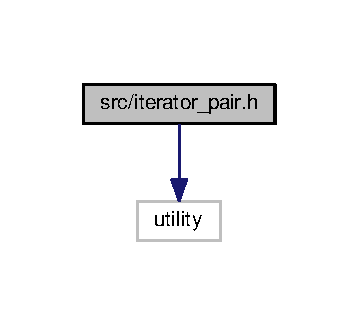
\includegraphics[width=172pt]{iterator__pair_8h__incl}
\end{center}
\end{figure}
This graph shows which files directly or indirectly include this file\+:
\nopagebreak
\begin{figure}[H]
\begin{center}
\leavevmode
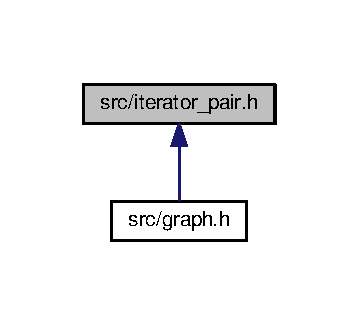
\includegraphics[width=172pt]{iterator__pair_8h__dep__incl}
\end{center}
\end{figure}
\subsection*{Classes}
\begin{DoxyCompactItemize}
\item 
class \hyperlink{classas_1_1iterator__pair}{as\+::iterator\+\_\+pair$<$ Iterator $>$}
\begin{DoxyCompactList}\small\item\em This class wraps a pair of begin and end iterators, and exposes them via \hyperlink{classas_1_1iterator__pair_a88c00afafd5ee4477b7ab2a1a89bb746}{begin()} and \hyperlink{classas_1_1iterator__pair_ae7cef6e91faecd20e6aebd2f21b29b41}{end()} function, which can be used in range-\/based for loops. \end{DoxyCompactList}\end{DoxyCompactItemize}
\subsection*{Namespaces}
\begin{DoxyCompactItemize}
\item 
 \hyperlink{namespaceas}{as}
\end{DoxyCompactItemize}
\subsection*{Functions}
\begin{DoxyCompactItemize}
\item 
{\footnotesize template$<$class Iterator $>$ }\\iterator\+\_\+pair$<$ Iterator $>$ \hyperlink{namespaceas_a4d4e0fb99b7cc564adaa85b693392070}{as\+::make\+\_\+iter} (std\+::pair$<$ Iterator, Iterator $>$ iters)
\begin{DoxyCompactList}\small\item\em Gives an \hyperlink{classas_1_1iterator__pair}{iterator\+\_\+pair} object constructed from the beginning and end iterators, given as a pair. \end{DoxyCompactList}\end{DoxyCompactItemize}

\hypertarget{random_8h}{}\section{src/random.h File Reference}
\label{random_8h}\index{src/random.\+h@{src/random.\+h}}
{\ttfamily \#include $<$random$>$}\newline
{\ttfamily \#include $<$functional$>$}\newline
{\ttfamily \#include $<$algorithm$>$}\newline
{\ttfamily \#include \char`\"{}containers.\+h\char`\"{}}\newline
Include dependency graph for random.\+h\+:\nopagebreak
\begin{figure}[H]
\begin{center}
\leavevmode
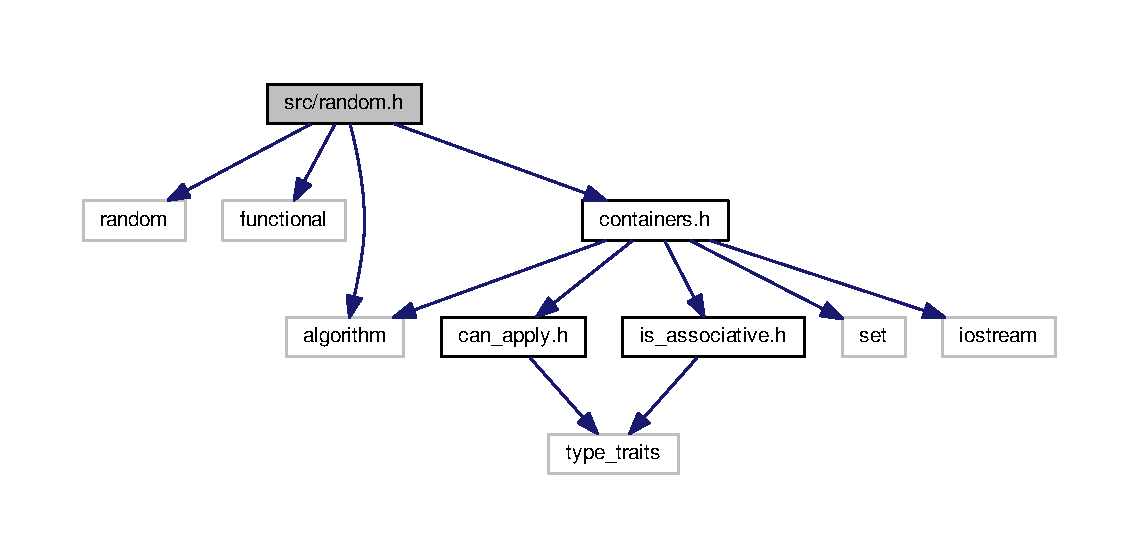
\includegraphics[width=350pt]{random_8h__incl}
\end{center}
\end{figure}
\subsection*{Namespaces}
\begin{DoxyCompactItemize}
\item 
 \hyperlink{namespaceas}{as}
\end{DoxyCompactItemize}
\subsection*{Functions}
\begin{DoxyCompactItemize}
\item 
std\+::mt19937 \hyperlink{namespaceas_a4c9b0919bddf60796e9cc81ecd7d5bb2}{as\+::get\+\_\+seeded\+\_\+mt} ()
\begin{DoxyCompactList}\small\item\em Gets a properly seeded Mersenne Twister prng. \end{DoxyCompactList}\item 
{\footnotesize template$<$class Container , class Prng  = std\+::mt19937$>$ }\\Container \hyperlink{namespaceas_a001b8303767234a8c93de5cb530a8f3d}{as\+::sample} (const Container container, typename Container\+::size\+\_\+type how\+\_\+many, Prng \&\&prng)
\begin{DoxyCompactList}\small\item\em Gets samples from a container. The samples are guaranteed to be unique. If we are requesting more samples than elements in the container, the request is ignored, and instead a random permutation of the container is returned. \end{DoxyCompactList}\item 
{\footnotesize template$<$class Container $>$ }\\Container \hyperlink{namespaceas_ab2b3e64b4dee388f0ec34e41ae0b3e98}{as\+::sample} (const Container container, typename Container\+::size\+\_\+type how\+\_\+many)
\begin{DoxyCompactList}\small\item\em Gets samples from a container. The samples are guaranteed to be unique. If we are requesting more samples than elements in the container, the request is ignored, and instead a random permutation of the container is returned. \end{DoxyCompactList}\end{DoxyCompactItemize}

%--- End generated contents ---

% Index
\backmatter
\newpage
\phantomsection
\clearemptydoublepage
\addcontentsline{toc}{chapter}{Index}
\printindex

\end{document}
